The top quark mass measurements in the di-lepton channel presented in Refs.~\cite{Aad:2015nba,AMaierPhD:2015,Aaboud:2016igd}
 use the template method.
 In this method, simulated distributions are constructed for different
 input values of the top quark mass, \mtin.
 The distributions (templates) per \mtin\ are then individually fitted to a
 suitable function. Using templates at different \mtin, it is verified that all
 parameters of the function linearly depend on $\mt=\mtin$. Consequently, this
 linearity is imposed in a combined fit to all templates.
%
 This fit fixes the theory prediction (i.e.~the parametrisation of the theory
 hypothesis) by determining all parameters of the function, except for \mt\ and
 the absolute normalisation.
%
 The former is to be determined from the data and represents the fit result, while
 the latter is left as a free parameter.
%
 We therefore follow the experimental procedure to neglect the absolute normalisation in the fit
 to avoid a dependence on the involved experimental determination of the total luminosity
 and detector efficiency.
%
 This choice makes the results of this study independent of the total cross section of
 the respective calculations, leaving shape changes of the differential distributions
 as the measure for \mt.
%
 Using those parameter values, a likelihood fit of this function to data is
 performed to obtain the value for \mt\ that best describes the data,
 namely \mtou, together with its statistical uncertainty.


 In experimental analyses, these templates are constructed at the detector
 level, i.e.~mimicking real data.
%
 Here, an analogous procedure is employed to
 assess the impact of different theory descriptions on
 the template method used to determine the top quark mass.
 In our analysis, the pseudo-data mimicking experimental data (i.e.~the data
 model) are always generated from those predictions, which are believed
 to be closest to real data, i.e.~those that are considered to give
 the ``better'' result.
%
 We simulate a data luminosity of $50/\mrm{fb}$.


 The sensitivity to the theoretical assumptions and their uncertainties is
 assessed by fits to one thousand pseudo-data sets created by random sampling from
 the underlying theory prediction.
%
 The layout of Figure~\ref{fig:LOvsNLO_NWA_decayLO} is representative for an
 entire set of figures presented in the following. For three different values
 of \mtin, each of these figures shows the observed difference of
 \mtou, the mass measured by the procedure, and \mtin, the mass used
 to generate the pseudo-data.
%
 The red/blue points correspond to the mean difference observed for all pseudo-data
 sets that are produced  as stated in the second line of the figure
 legends,  and analysed with the template fit functions (the theory
 hypothesis), denoted by ``calibration''  in the legend for
 the red/blue points.
 The uncertainty per point is statistical only and corresponds to
 the expected experimental uncertainty for the assumed data luminosity.
 The points are displaced on the horizontal axis to ensure better
 visibility in the case of overlapping bands.
The horizontal lines stem from a fit of the three points to a
 constant, displaying the {\em average} offset.
  The values given are the (individual) offsets together with their
 statistical uncertainties.
%
 The bands indicate the effect of the scale variations on the measured \mt.
 They are obtained by replacing the central-scale pseudo-data by those
 derived from
 the associated samples, which were calculated using the varied scales.

 The ranges of the fits have been chosen on a plateau of good fit performance and high mass sensitivity.
%
The ranges of choice are
\begin{align}
&40\gev\leq \mlb\leq 160\gev\;,\label{eq:fitranges}\\
&80\gev\leq \mtwo\leq 180\gev\;.\nonumber
\end{align}
Note that for the $\nlops$ calculations employing the $\mu_{t\bar t}$
scale, we used a fit range of $50\gev\leq \mlb\leq 150\gev$.


\boldmath
\subsection{Fit results for $m_{lb}$}
\unboldmath

\begin{figure}[tbp!]
  \centering
  \begin{subfigure}{0.495\textwidth}
    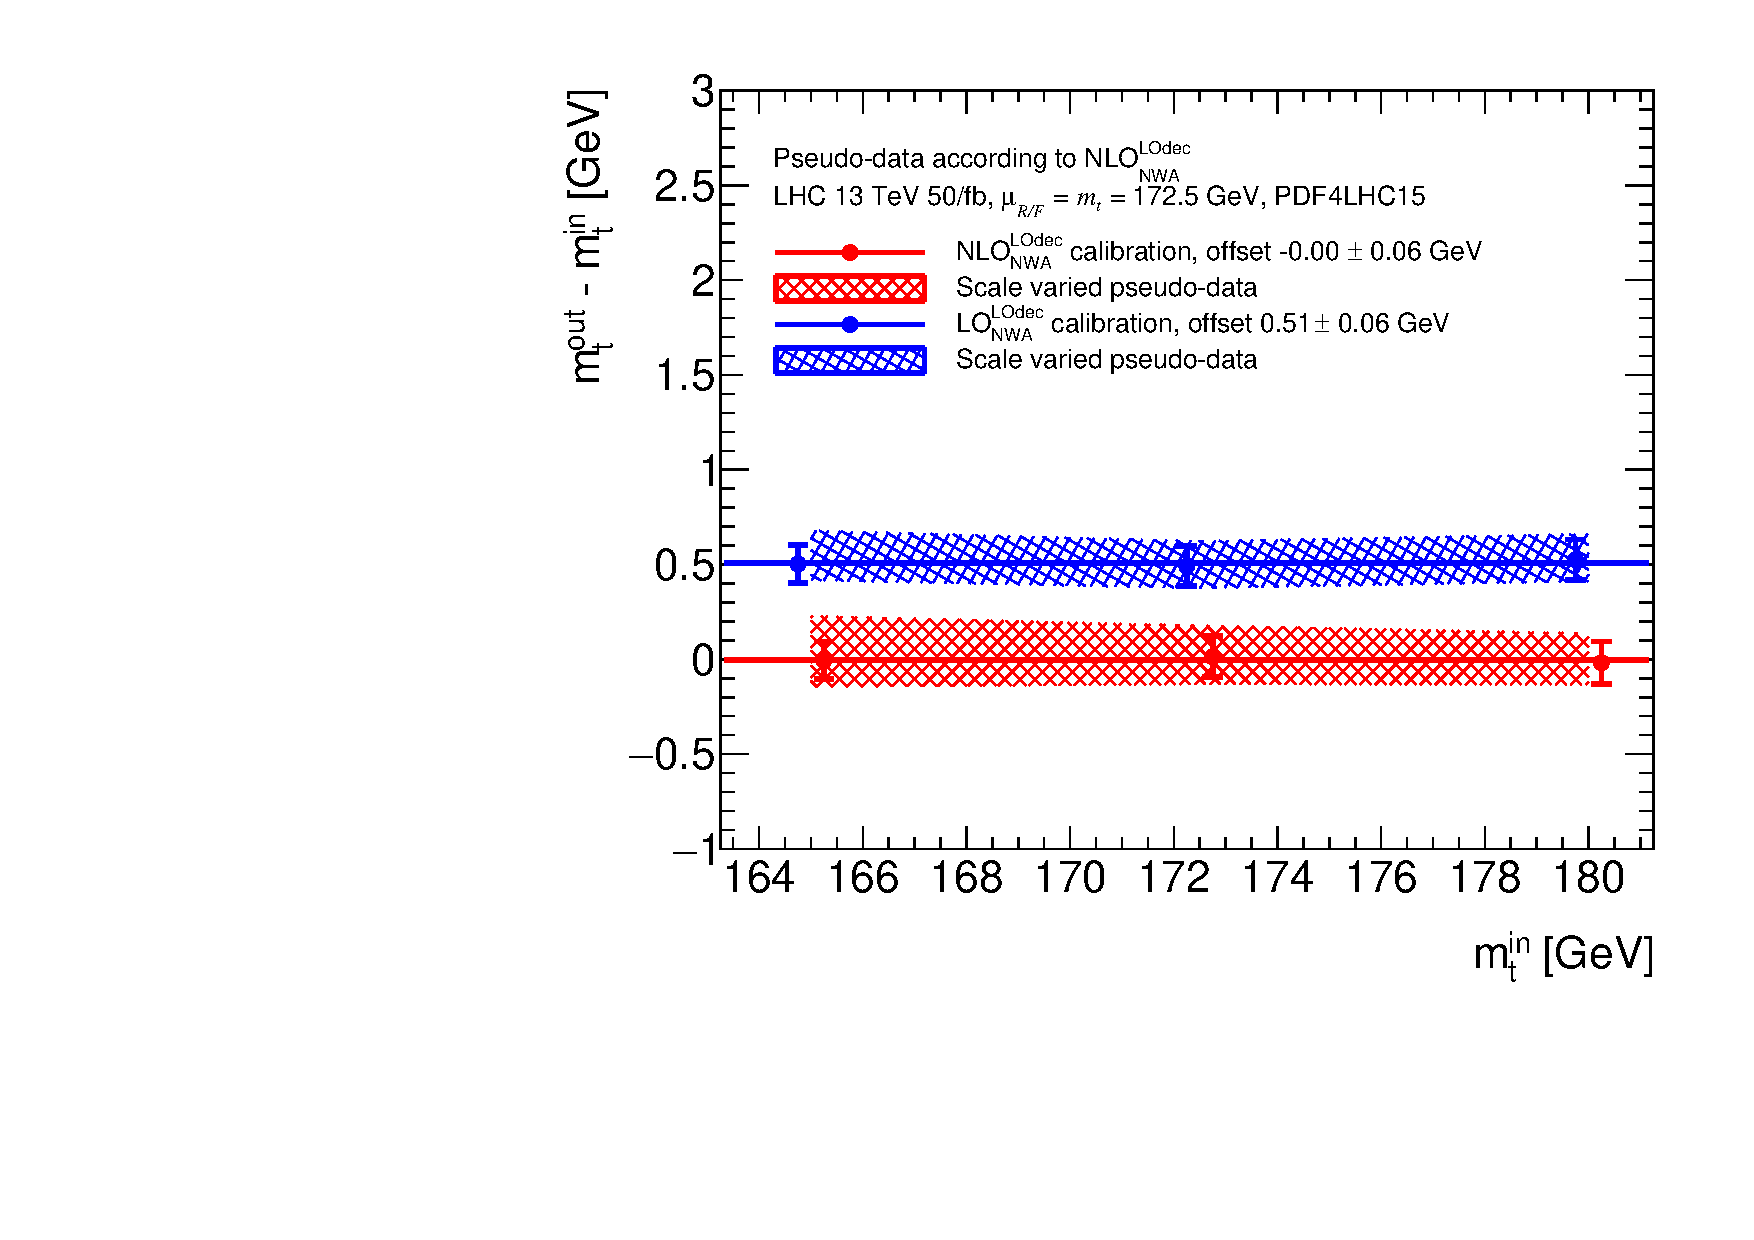
\includegraphics[width=\textwidth]{{plots/mlb_f1_13TeVstd_NLO_vs_LO_pexpseed0}.pdf}
    %\caption{Factorised, production LO versus NLO, decay LO. }
    \vspace{\TwoFigBottom em}
    \caption{\label{fig:LOvsNLO_NWA_decayLO}}
  \end{subfigure}
  \hfill
  \begin{subfigure}{0.495\textwidth}
    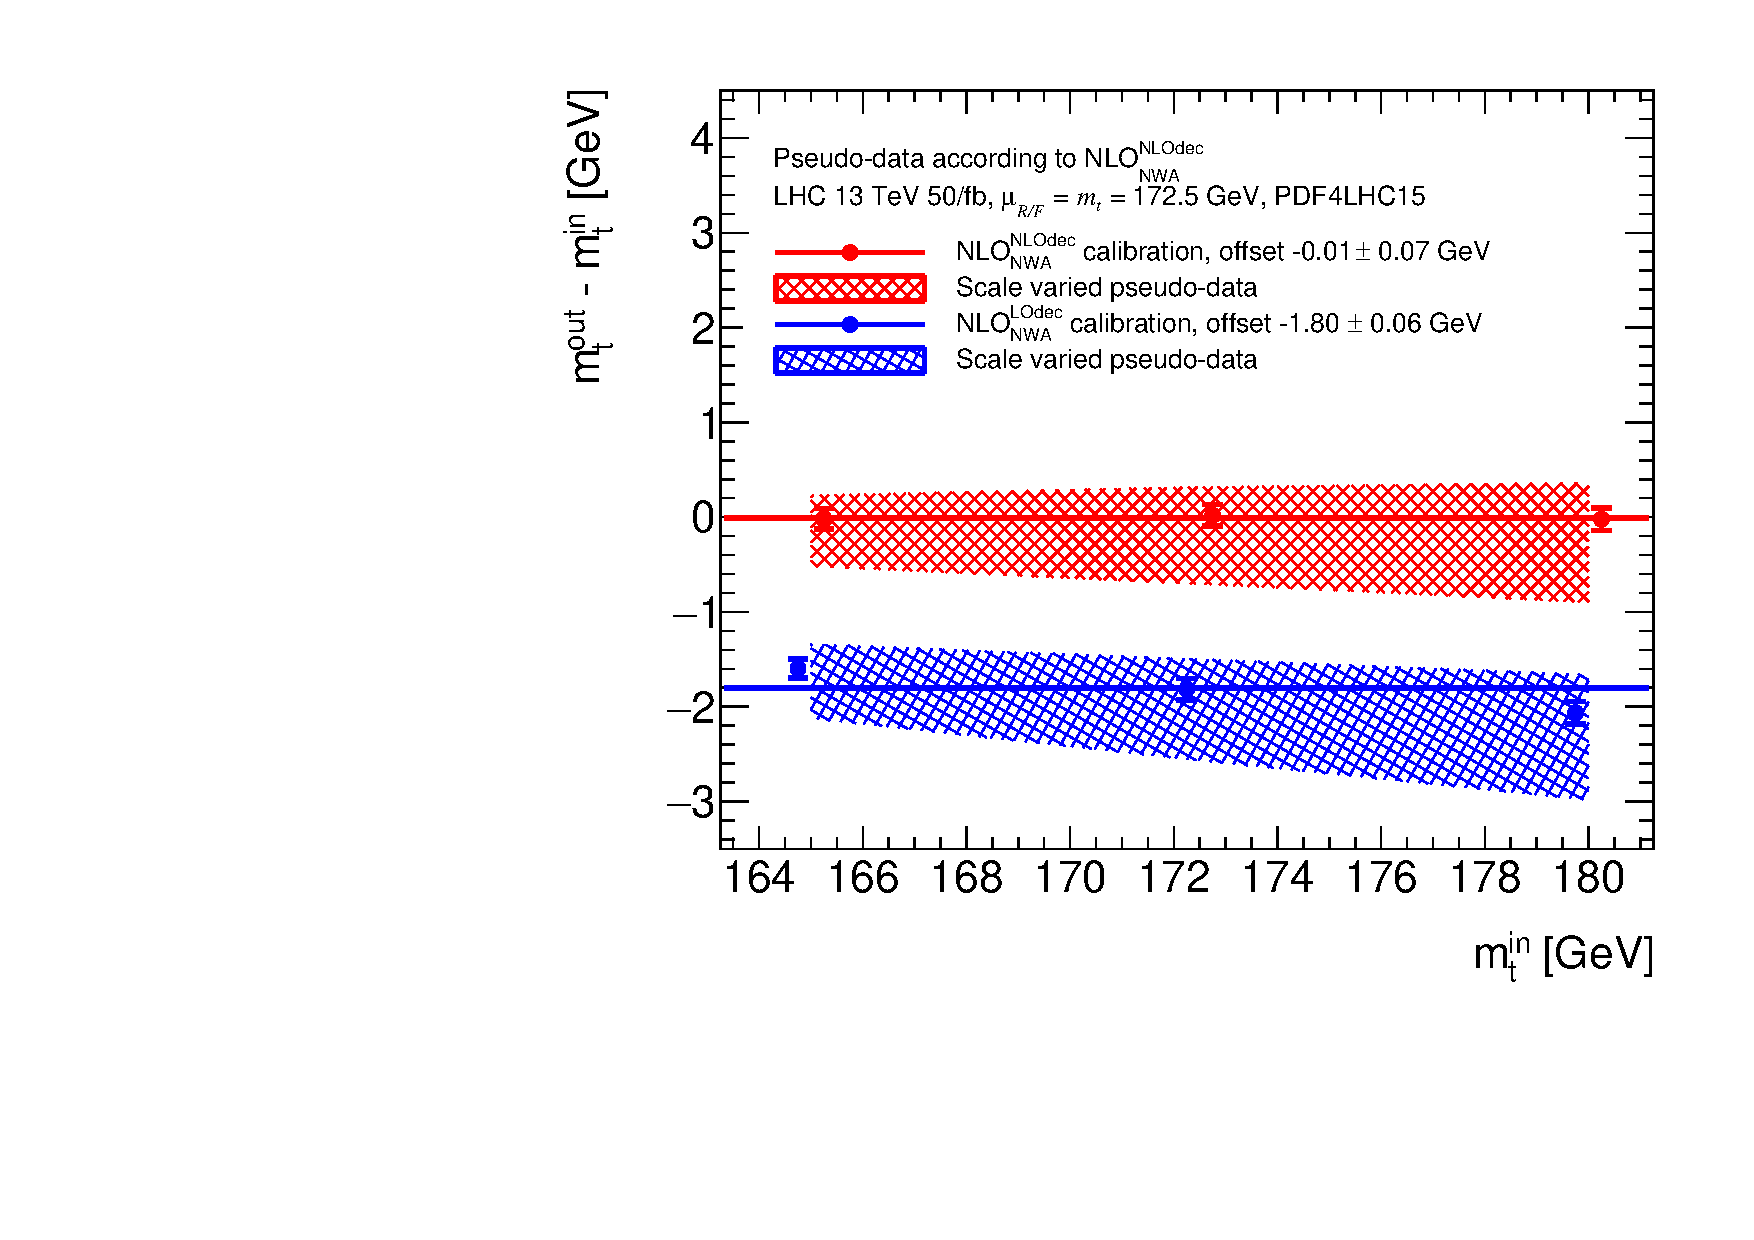
\includegraphics[width=\textwidth]{{plots/mlb_f1_13TeVstd_decay_order_pexpseed0}.pdf}
    %\caption{Factorised, production NLO, decay LO versus NLO.}
    \vspace{\TwoFigBottom em}
    \caption{\label{fig:NLO_NWA_decayLOvsNLO}}
  \end{subfigure}
  \caption{\label{fig:NWA}%
    Results of the top quark mass determination using the observable $m_{lb}$
    and (a) pseudo-data generated according to the factorised
    approach with $\lodec$, showing the effect of changing
    the perturbative order in the production process only, and (b)
    pseudo-data obtained from the factorised approach with
    $\nlodec$, showing the effect of changing the perturbative order
    in the decay process only.}
\end{figure}

Figure~\ref{fig:LOvsNLO_NWA_decayLO} shows results of a fit where the pseudo-data have been generated using the factorised approach with $\lodec$.
The fit has been performed once with $\lolo$ as the theory model (blue) and once with $\lodec$ (red).
The vanishing offset (i.e.~it is compatible with zero) for the red lines (here and in all the following figures) proves that the method is closed, i.e.~it finds the input value when the pseudo-data and the calibration coincide.
The offset between the blue and red lines in
Fig.~\ref{fig:LOvsNLO_NWA_decayLO} shows the effect of changing the
perturbative order of the {\em production} process in the theory
model. The offset of  $0.51\pm 0.06\,\gev$
demonstrates that these corrections have an impact
on the mass determination at the level of the present experimental uncertainties. As the fits are based on
normalised differential cross sections, the bands are sensitive to
shape differences induced by the scale variations, rather than to their
overall magnitudes.

Figure~\ref{fig:NLO_NWA_decayLOvsNLO} shows results of a fit where the
pseudo-data have been generated using the factorised approach based on
the $\nlodec$, i.e.~the NWA at NLO, while the theory models differ in
the {\em decay} order only. We observe that the effect of an
${\cal O}(\as{})$ change in the perturbative order of the decay is
more significant than changing the order in the production process.
The offset stemming from the former amounts to $-1.80\pm0.06\gev$, while
switching from LO to NLO in the description of the production process
yields an offset of $0.51\pm0.06\gev$ (cf.~Fig.~\ref{fig:LOvsNLO_NWA_decayLO}).
In addition, the size of the uncertainty bands increases because the NLO corrections to the decay lead to non-uniform scale variation bands.

Figure~\ref{fig:NLO_NWA_decayNLO} shows the effect of changing the
perturbative order in both the production and decay process.
Comparing Figs.~\ref{fig:NWA} and~\ref{fig:NLO_NWA_decayNLO}, we observe that,
within the statistical uncertainties,  the offset in Fig.~\ref{fig:NLO_NWA_decayNLO} coincides with
the sum of the offsets in Figs.~\ref{fig:LOvsNLO_NWA_decayLO} and
\ref{fig:NLO_NWA_decayLOvsNLO}, as is expected for the factorised approach.
%
Figure~\ref{fig:fullNLO} shows results of a fit where the pseudo-data
have been generated using the $\nlofull$ calculation, and the
calibrations are based on the $\nlofull$ and $\lofull$
descriptions. While the uncertainty bands are comparable to the
factorised case that uses pseudo-data based on $\nlodec$
(Fig.~\ref{fig:NLO_NWA_decayNLO}), the offset increases from
$-1.38\pm0.07\gev$ to $-1.52\pm0.07\gev$.
While this increase in the offset is not conclusive when taking the
statistical uncertainty into account, it still is an indication of the
trend that the inclusion of a richer set of corrections leads to larger
offsets.

\begin{figure}[tbp!]
  \centering
  \begin{subfigure}{0.495\textwidth}
    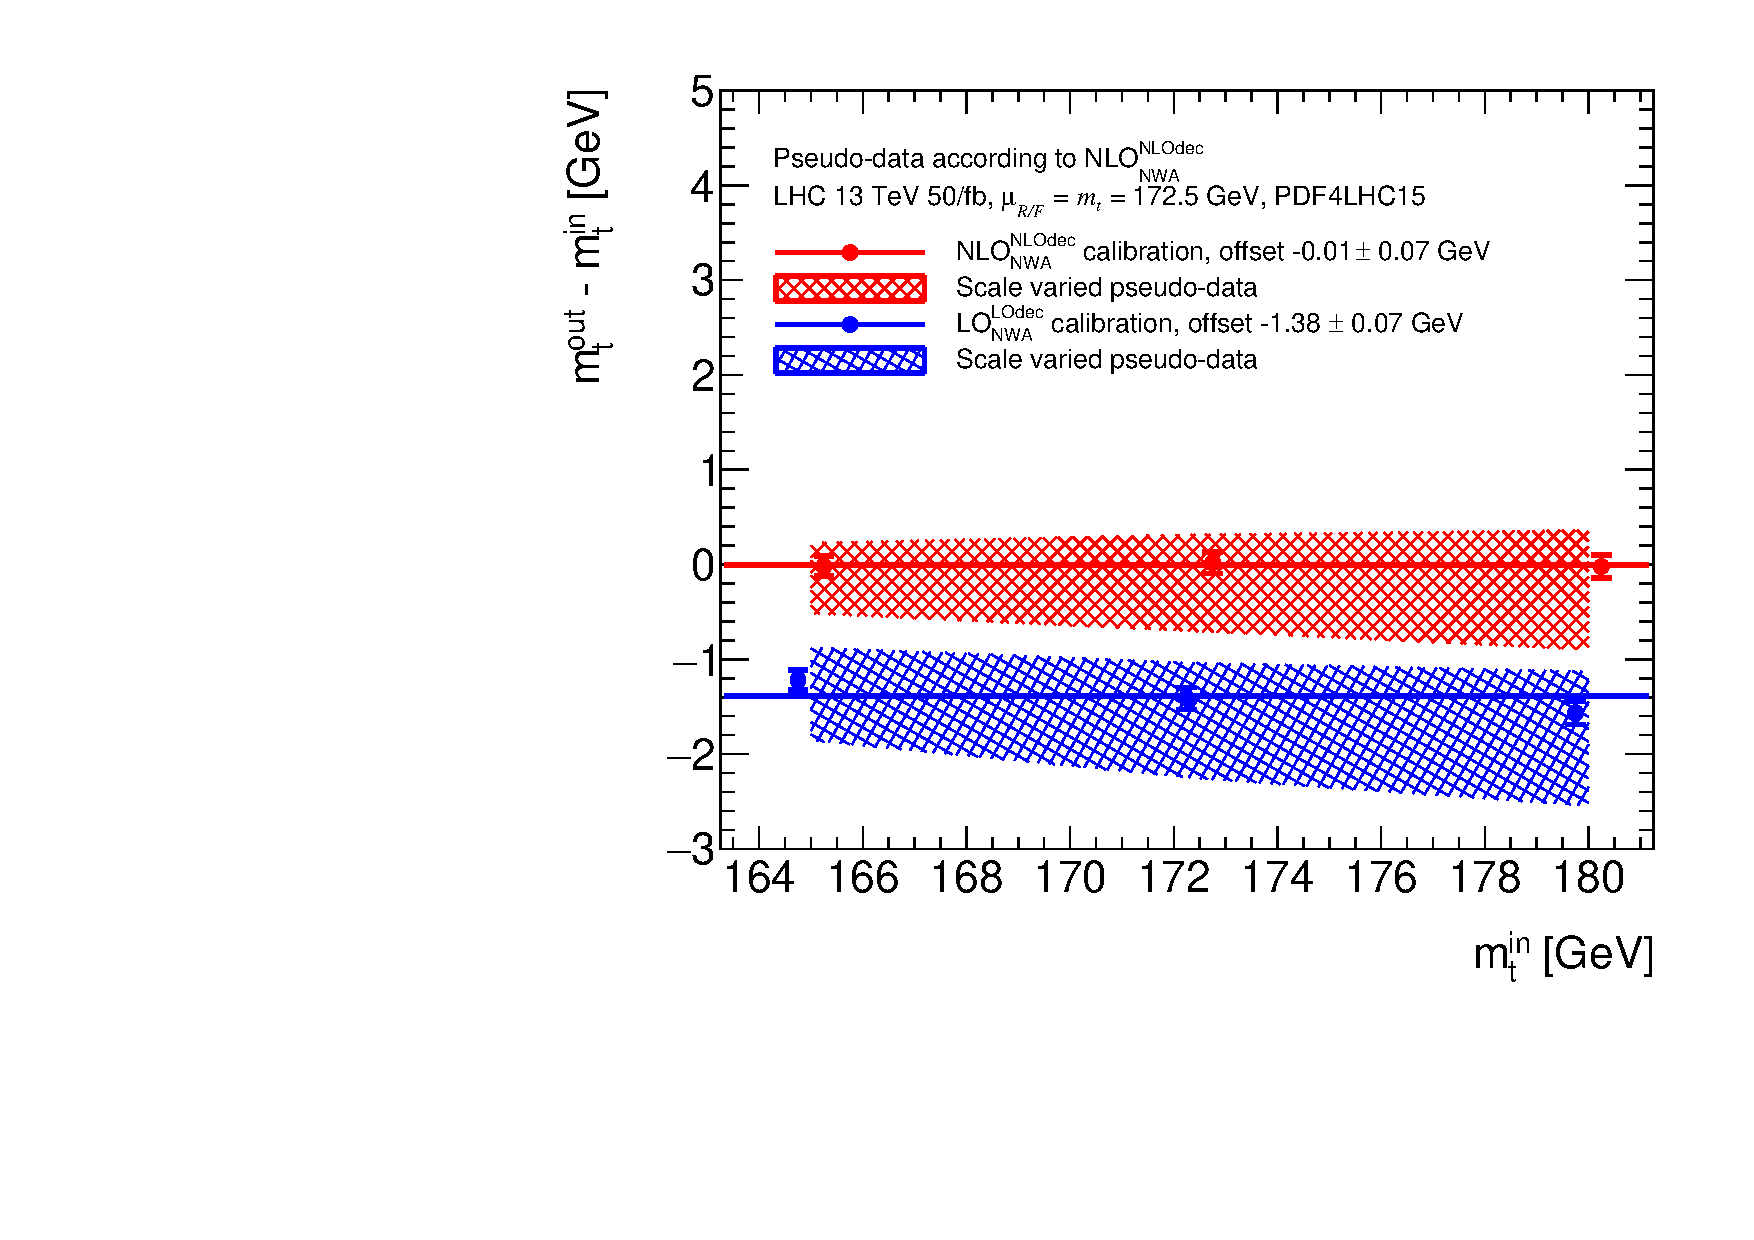
\includegraphics[width=\textwidth]{{plots/mlb_f1_13TeVstd_NLOn_vs_LO_pexpseed0}.pdf}
    \vspace{\TwoFigBottom em}
    \caption{\label{fig:NLO_NWA_decayNLO}}
  \end{subfigure}
  \hfill
  \begin{subfigure}{0.495\textwidth}
    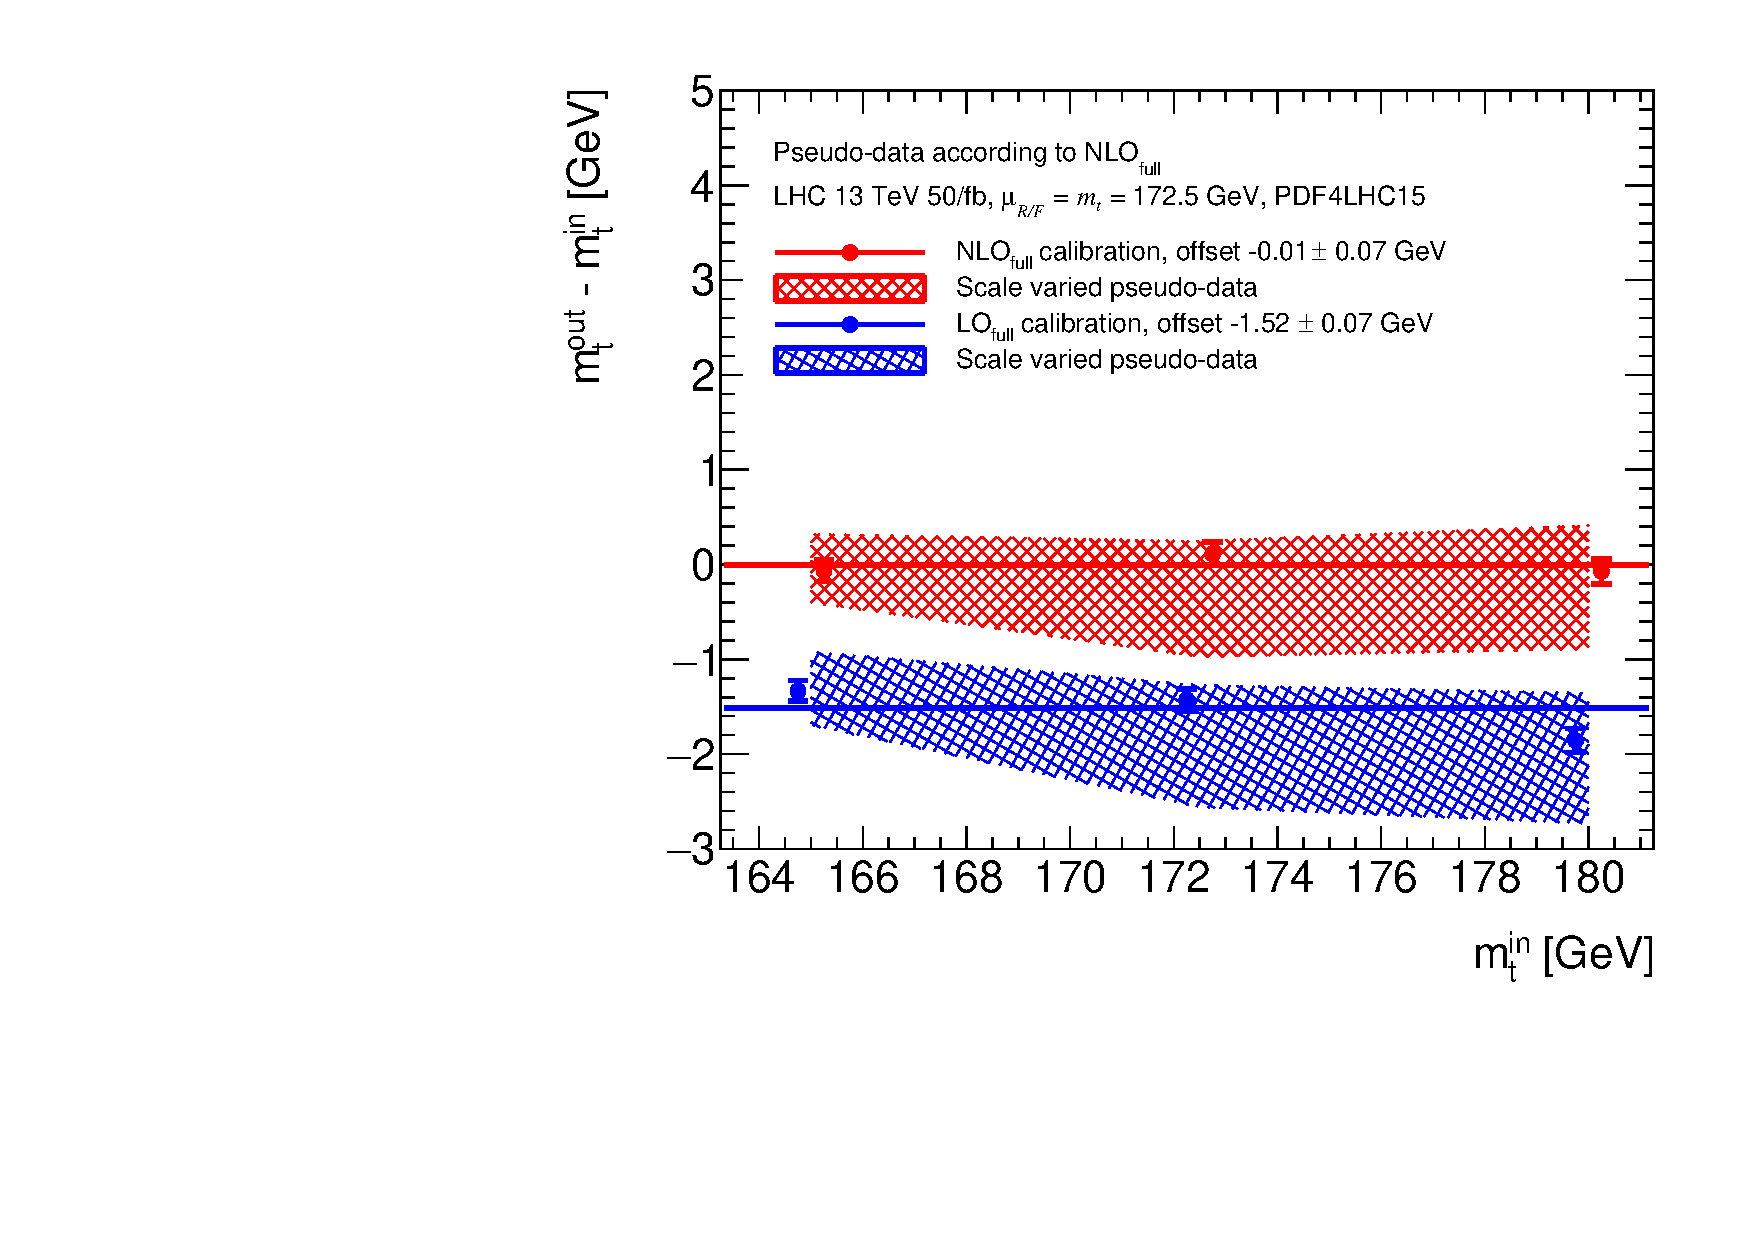
\includegraphics[width=\textwidth]{{plots/mlb_f1_13TeVstd_WWbb_diff_pexpseed0}.pdf}
    \vspace{\TwoFigBottom em}
    \caption{\label{fig:fullNLO}}
  \end{subfigure}
  \caption{\label{fig:NWAboth}%
    Results of the top quark mass determination using the observable $m_{lb}$
    and (a) pseudo-data generated according to the factorised
    approach with $\nlodec$, showing the effect of changing
    the perturbative order in both the production and decay process,
    and (b) pseudo-data derived from $\nlofull$ distributions. In both
    cases, the focus is on the comparison of LO versus NLO calibrations.}
\end{figure}

In Fig.~\ref{fig:NLO_WWbb_vs_NWA_decayNLO}, we again use pseudo-data
generated according to $\nlofull$,
this time comparing the fit based on the full NLO calibration to the one
obtained with the $\nlodec$ calibration representing the factorised NLO
approach.
We see that the offset of $0.83\pm0.07\gev$ is smaller in magnitude
than in Fig.~\ref{fig:fullNLO}, and goes in the opposite direction.
%
This indicates that the non-factorisable contributions are suppressed
in the fit range, since the NWA, with the corrections to the decay 
included, is a better approximation than $\lofull$ only.

In Fig.~\ref{fig:WWbb_vs_PS_NLO}, we replace the $\nlodec$ calibration 
by the one from the $\nlops$ prediction.
% 
We observe an offset of $-0.09\pm0.07\gev$, which is
surprisingly small compared to that given in
Fig.~\ref{fig:NLO_WWbb_vs_NWA_decayNLO}. It is expected
that the two NWA-based descriptions, both including 
the leading radiation in the decay, lead to quite
similar results. However, the $\nlops$ simulation differs from the
$\nlodec$ calculation in a number of points.
While $\nlops$ falls short of describing the top quark
decay beyond the soft limit owing to the absence of decay matrix-element
corrections, the parton shower approach generates a very different,
more complete QCD radiation pattern
as a result of including resummation effects in the production
as well as the decay of the top quarks. This means that the two stages
of $t\bar t$\/ production and decay are not  factorised in
exactly the same way as in the $\nlodec$ calculation. These
differences explain why the offset in
Fig.~\ref{fig:NLO_WWbb_vs_NWA_decayNLO} is different from the
one in Fig.~\ref{fig:WWbb_vs_PS_NLO}.
%
In fact, as can be seen from Figs.~\ref{fig:scalevar_mlb} as well
as~\ref{fig:mlb_scalevar_nwa}, the emission pattern and resummation
effects of the $\nlops$ case are relevant at lower $\mlb$ values and
in particular around (and above) the kinematic edge, and lead to a
shape of the \mlb distribution, which differs from the fixed-order
$\nlodec$ case. Especially for the $\mlb\sim140\gev$ region, we notice
that the agreement between $\nlops$ and $\nlofull$ is better than
between $\nlops$ and $\nlodec$. This is an
indication that in this region, resummation effects are more important
than the inclusion of the radiative correction in the decay.
The nearly vanishing mass offset shown in Fig.~\ref{fig:WWbb_vs_PS_NLO} occurs
due to the fact that the shapes of $\nlops$ and $\nlofull$ do
not differ significantly in most of the fit range, despite their different theoretical content.

\begin{figure}[tbp!]
\centering
\begin{subfigure}{0.495\textwidth}
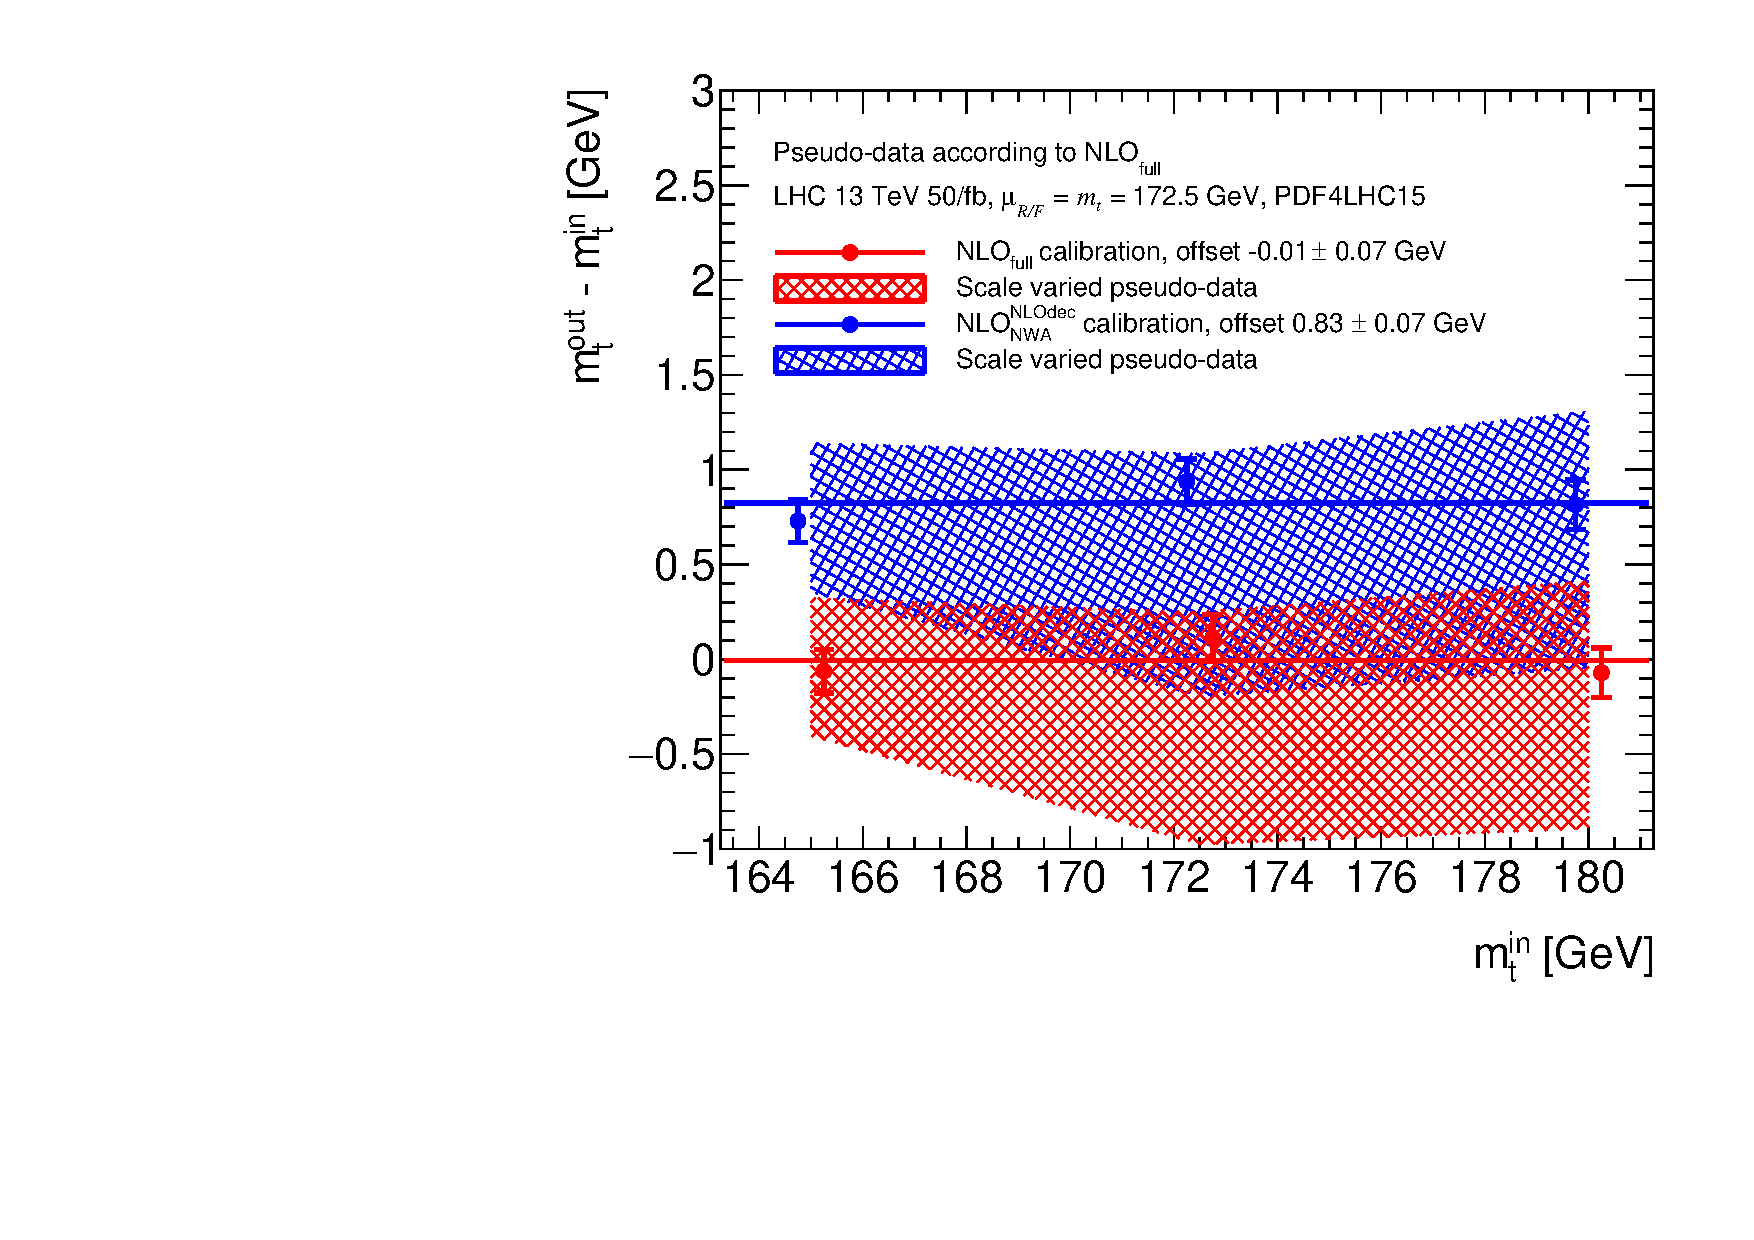
\includegraphics[width=\textwidth]{{plots/mlb_f1_13TeVstd_WWbb_vs_ttbar_pexpseed0}.pdf}
\vspace{\TwoFigBottom em}
\caption{\label{fig:NLO_WWbb_vs_NWA_decayNLO}}
\end{subfigure}
\hfill
\begin{subfigure}{0.495\textwidth}
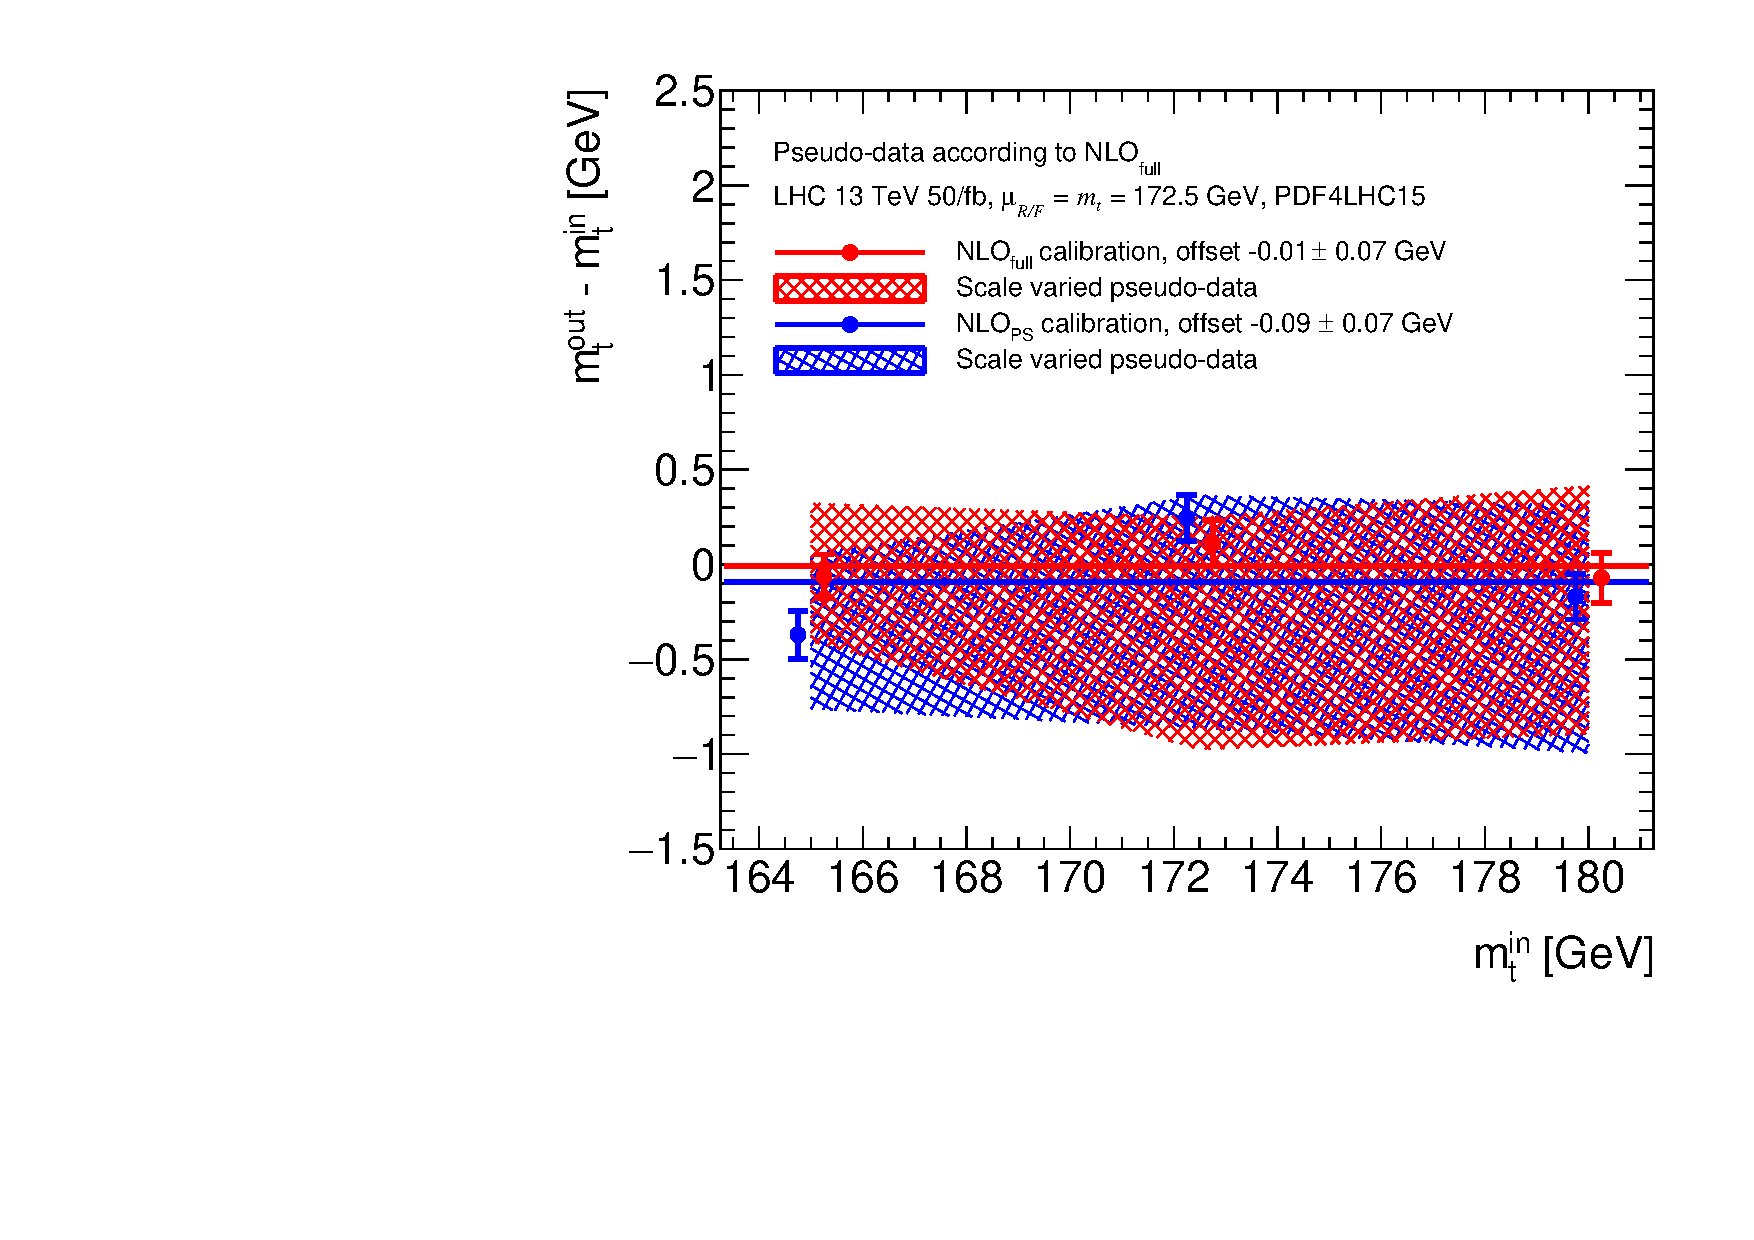
\includegraphics[width=\textwidth]{{plots/mlb_f1_13TeVstd_WWbb_NLO_vs_PS_pexpseed0}.pdf}
\vspace{\TwoFigBottom em}
\caption{\label{fig:WWbb_vs_PS_NLO}}
\end{subfigure}
\caption{\label{fig:NLO_WWbb_vs}%
  Top quark mass determination results for the observable $m_{lb}$
  comparing pseudo-data generated according to the $\nlofull$
  predictions with (a) the $\nlodec$ calibration and (b) the $\nlops$
  calibration.}
\end{figure}

In Fig.~\ref{fig:NLO_PS_vs}, 
we use pseudo-data generated according to the $\nlops$ prediction
using the scale setting $\mu_F=\mu_R=m_t$. The related
scale variations have been obtained by employing the
$\mu_F\mu_R\as{\mathrm{PS}}$ scheme as described at the end of
Section~\ref{subsec:input}. 
By comparing to Fig.~\ref{fig:LOvsNLO_NWA_decayLO}, 
we observe that the uncertainty bands of $\nlops$ are smaller than the
ones for $\lodec$. However, for the theory models relying on NLO decays,
as shown in Fig.~\ref{fig:NLO_NWA_decayLOvsNLO} for $\nlodec$
and in Fig.~\ref{fig:fullNLO} for $\nlofull$, the bands are much wider.
Hence, we expect that adding a parton shower to the $\nlofull$
calculation, the bands would persist or be only slightly reduced,
analogous to the LO decay situation discussed above.

Unlike the case presented in Fig.~\ref{fig:WWbb_vs_PS_NLO}, the direct
comparison between results from the NWAs and $\nlops$ produces
non-vanishing mass shifts.
If we analyse the $\nlops$ pseudo-data using the
fixed-order $\lodec$ calibration, we find a mass offset of
$-0.92\pm0.07\gev$ as shown in Fig.~\ref{fig:PS_vs_ttbar_NLO}. This
indicates that the parton shower emissions (in both stages),
supplementing the NLO accurate $t\bar t$ production, have a
considerable impact on the results.
%
In addition, a significant dependence of the $\lodec$ calibration offset
on the top quark mass is observed,
i.e.~the blue points are inconsistent with the constant fit.
%
This implies that the $\nlops$ \mlb\ distribution has a weaker
dependence on the top quark mass than the one generated by $\lodec$.
%
Turning to Fig.~\ref{fig:PS_vs_ttbar_NLO_nlodc}, we show the case
where the $\nlops$ pseudo-data have been confronted with the
improved fixed-order model $\nlodec$. For this case, we would expect a
pseudo-data-theory agreement which is better than the one seen in
Fig.~\ref{fig:PS_vs_ttbar_NLO}, since
both the $\nlops$ and the $\nlodec$ description contain the major
contributions to describe the extra emission in the top quark decays.
However, the offset of
$0.96\pm0.07\gev$ is similar in size (while opposite in direction)
compared to the LO decay case shown in Fig.~\ref{fig:PS_vs_ttbar_NLO}.
This is consistent with the offset differences shown in Table~\ref{tab:offset}, 
for example subtracting the offset given in Fig.~\ref{fig:NLO_NWA_decayLOvsNLO}
 from the one in Fig.~\ref{fig:PS_vs_ttbar_NLO}, 
or alternatively the one in Fig.~\ref{fig:WWbb_vs_PS_NLO} from the one
in Fig.~\ref{fig:NLO_WWbb_vs_NWA_decayNLO}.

\begin{figure}[tbp!]
\centering
\begin{subfigure}{0.495\textwidth}
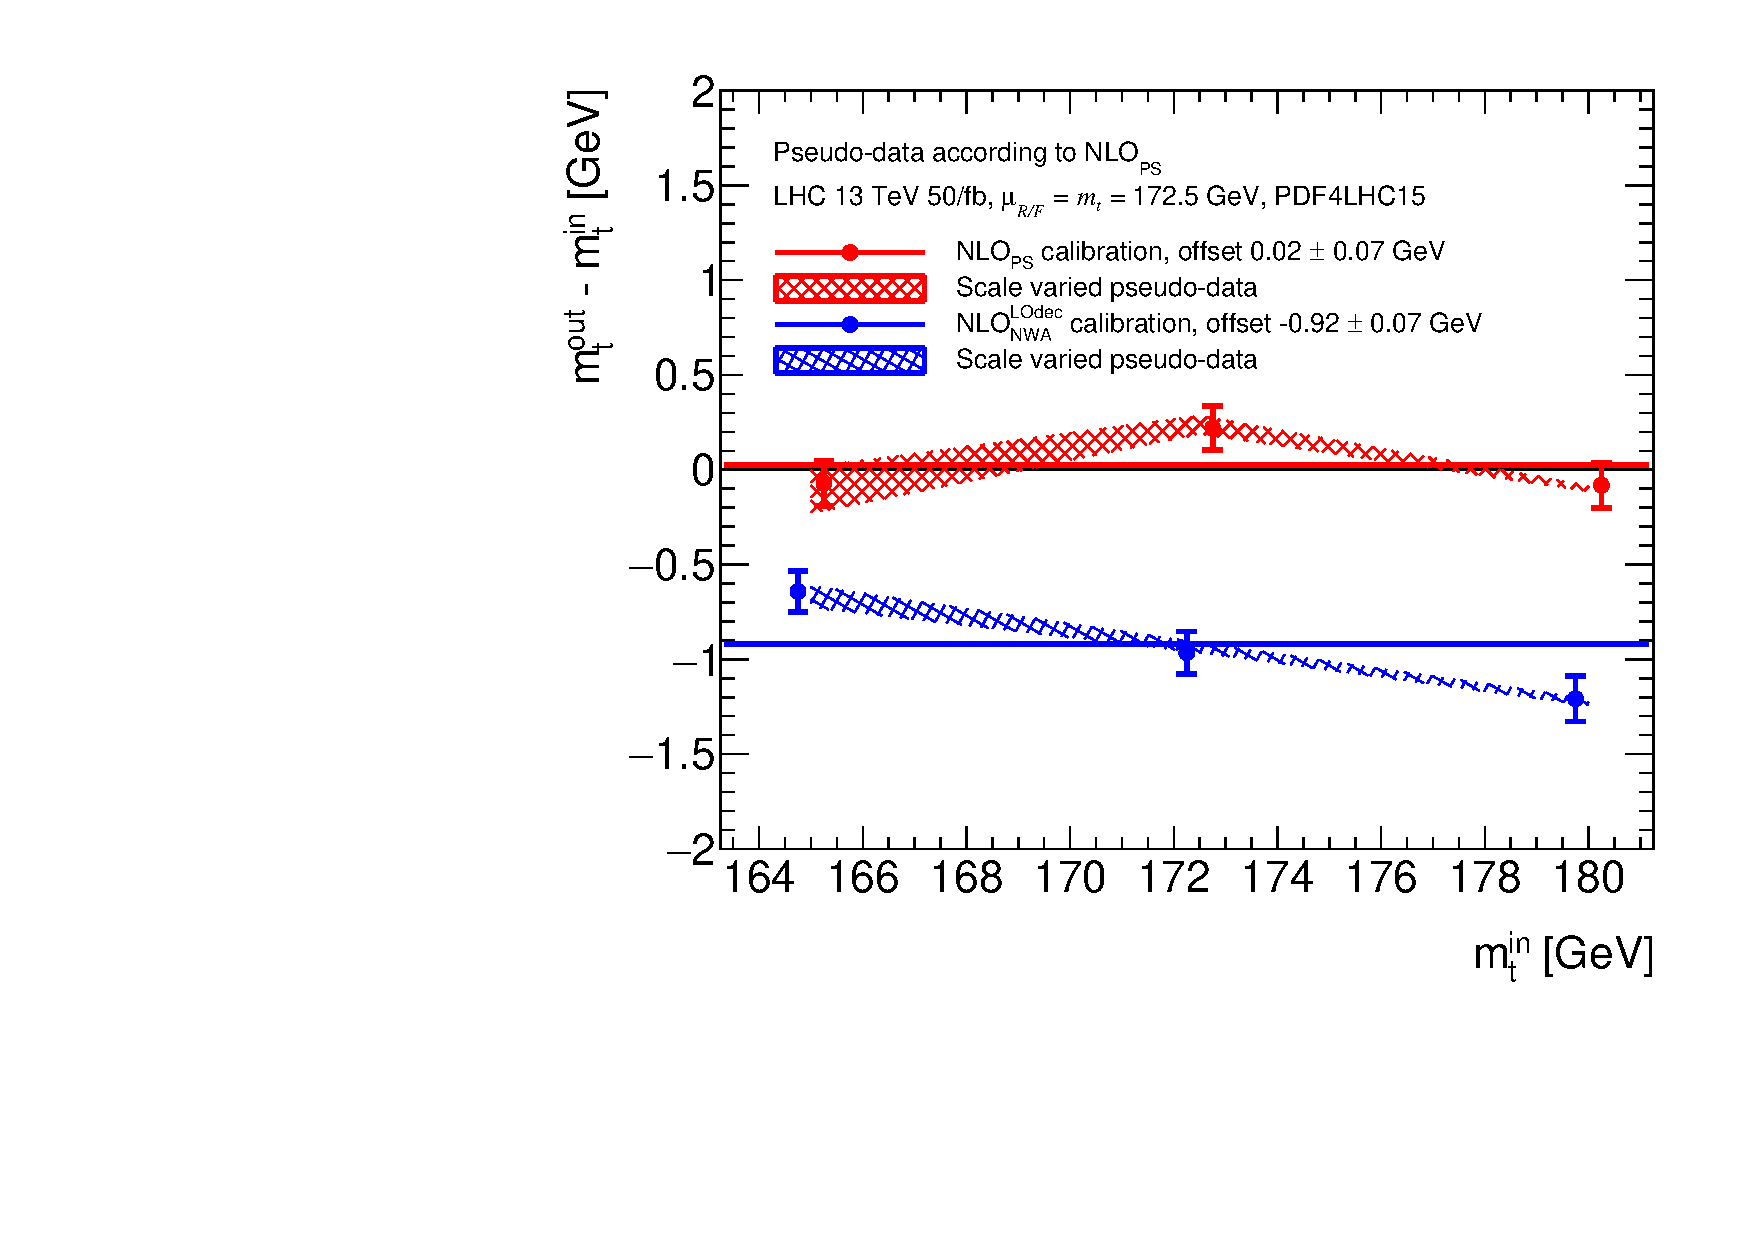
\includegraphics[width=\textwidth]{{plots/mlb_f1_13TeVstd_PS_vs_ttbar_NLO_pexpseed0}.pdf}
\vspace{\TwoFigBottom em}
\caption{\label{fig:PS_vs_ttbar_NLO}}
\end{subfigure}
\hfill
\begin{subfigure}{0.495\textwidth}
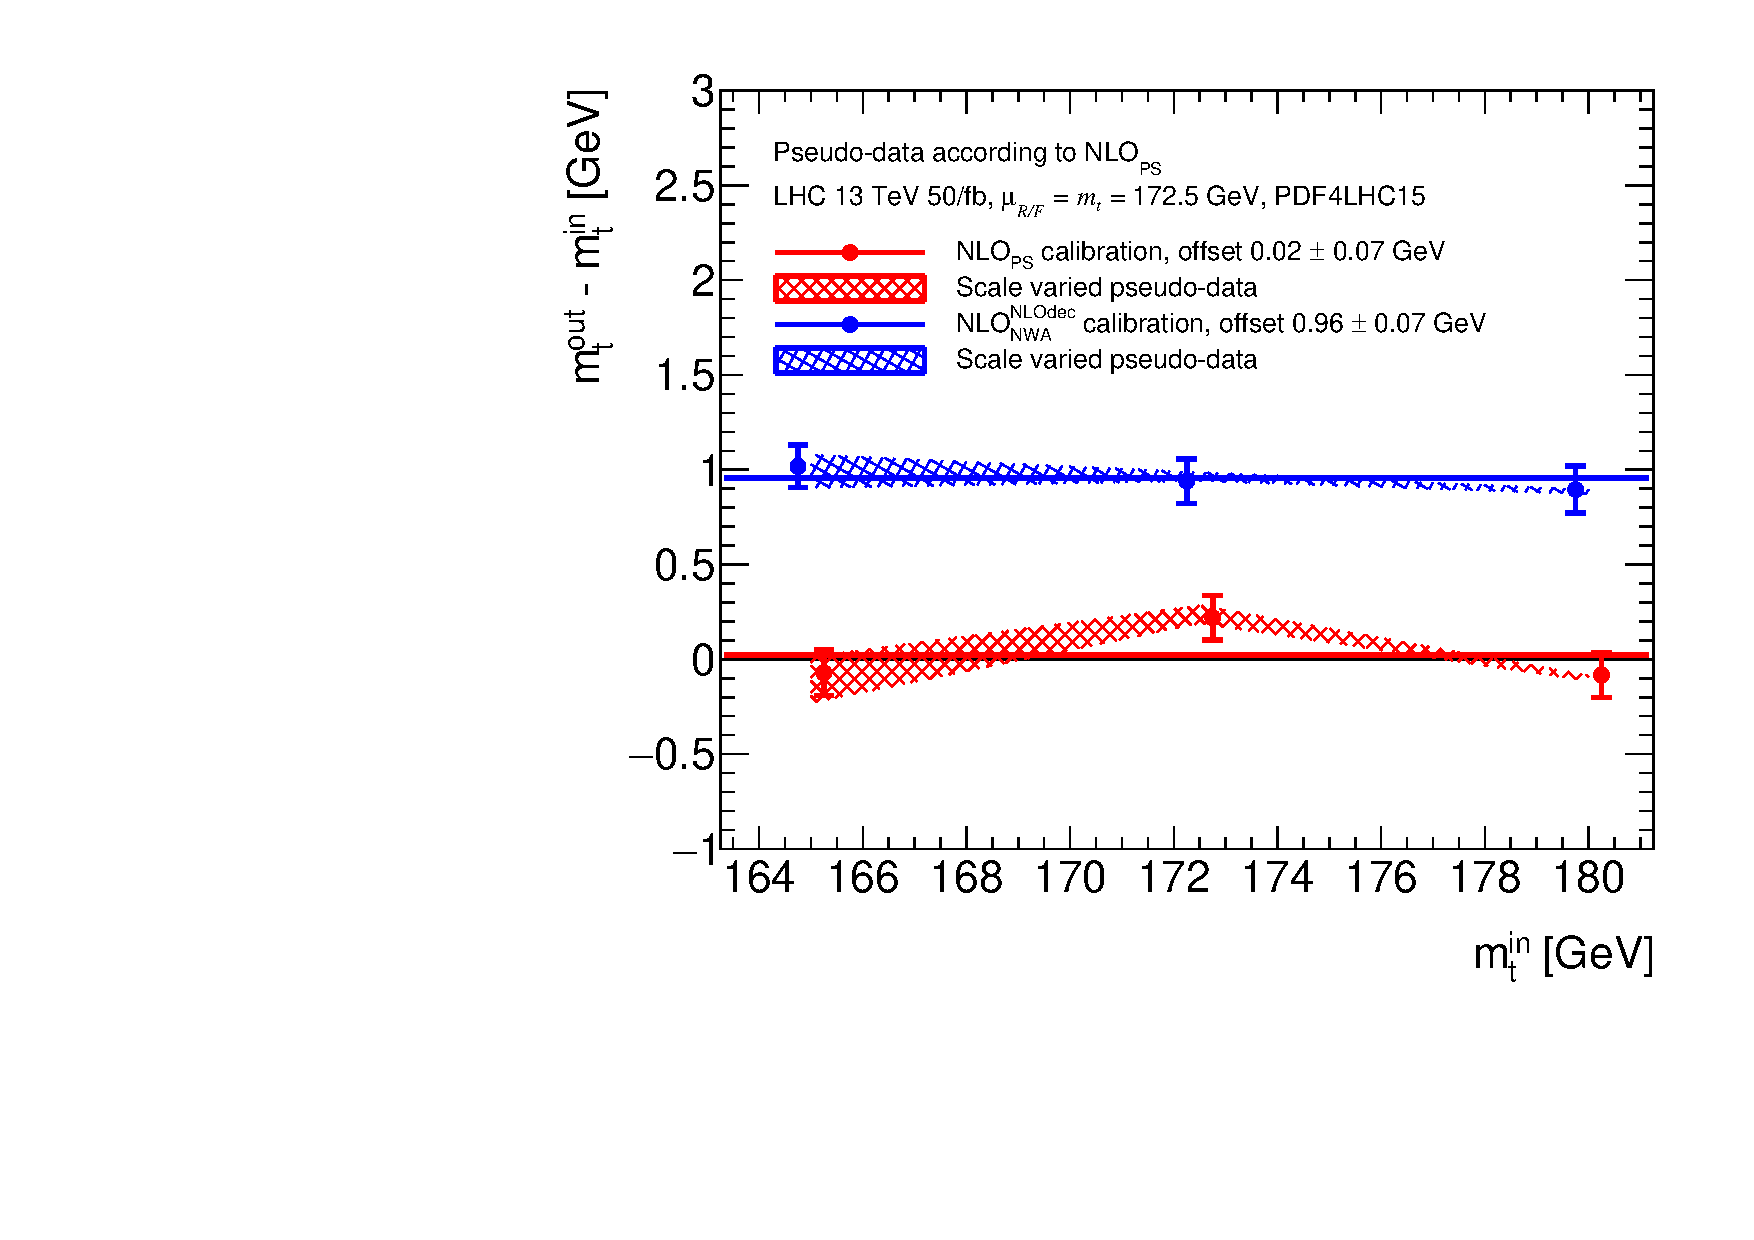
\includegraphics[width=\textwidth]{{plots/mlb_f1_13TeVstd_PS_vs_ttbar_NLO_nlodc_pexpseed0}.pdf}
\vspace{\TwoFigBottom em}
\caption{\label{fig:PS_vs_ttbar_NLO_nlodc}}
\end{subfigure}
\caption{\label{fig:NLO_PS_vs}%
  Top quark mass determination results for the observable $m_{lb}$
  comparing pseudo-data generated according to the $\nlops$
  predictions with  (a) the $\lodec$ calibration and (b) the $\nlodec$ calibration.}
\end{figure}

Further investigations are needed to understand the source of the 
mass shift observed in  Fig.~\ref{fig:PS_vs_ttbar_NLO_nlodc}. Based on
the current findings, we cannot conclude whether it
originates from ($i$)~the inclusion of resummation effects, or
($ii$)~genuine differences in incorporating the %${\cal O}(\as{})$~corrections
fixed-order QCD corrections to the production and decay of the top
quark pairs, or both.
The different radiation
patterns generated by $\nlops$ and $\nlodec$ do not allow for a strict,
same-level comparison between the two approaches, but reducing the
amount of radiation produced by $\nlops$ is expected to bring them closer to
each other, and to diminish the role of resummation effects.

There is no unique way of limiting the scope of the resummation.
To control the generation of a reduced branching pattern, we use an approach where each showering process
can be terminated after a (given) fixed number of emissions, denoted
by $n_\mrm{max}$. For our study, we rely on the fully factorised
version of combining the subshowers, i.e.~we separately restrict the
number of emissions to no more than $n$ ($\nprod=\ndec=n$) in each
subshower (the primary one evolving the $t\bar t$ production and the
secondary one evolving the decays). %(production plus both decays).
The combination of one-emission production and decay showers
($\nprod=\ndec=1$) can then be used to emulate the $\nlodec$
calculation, which enables us to approximately separate effects ($i$)
from ($ii$).
In addition, comparing the restricted and full $\nlops$ prescriptions
will provide us with a qualitative
estimate of the impact of the full resummation.
Starting from $\nprod=1$ and $\ndec=1$, we can successively restore
the full shower by incrementing the number of emissions.

\begin{figure}[t!]
\centering
\begin{subfigure}{0.495\textwidth}
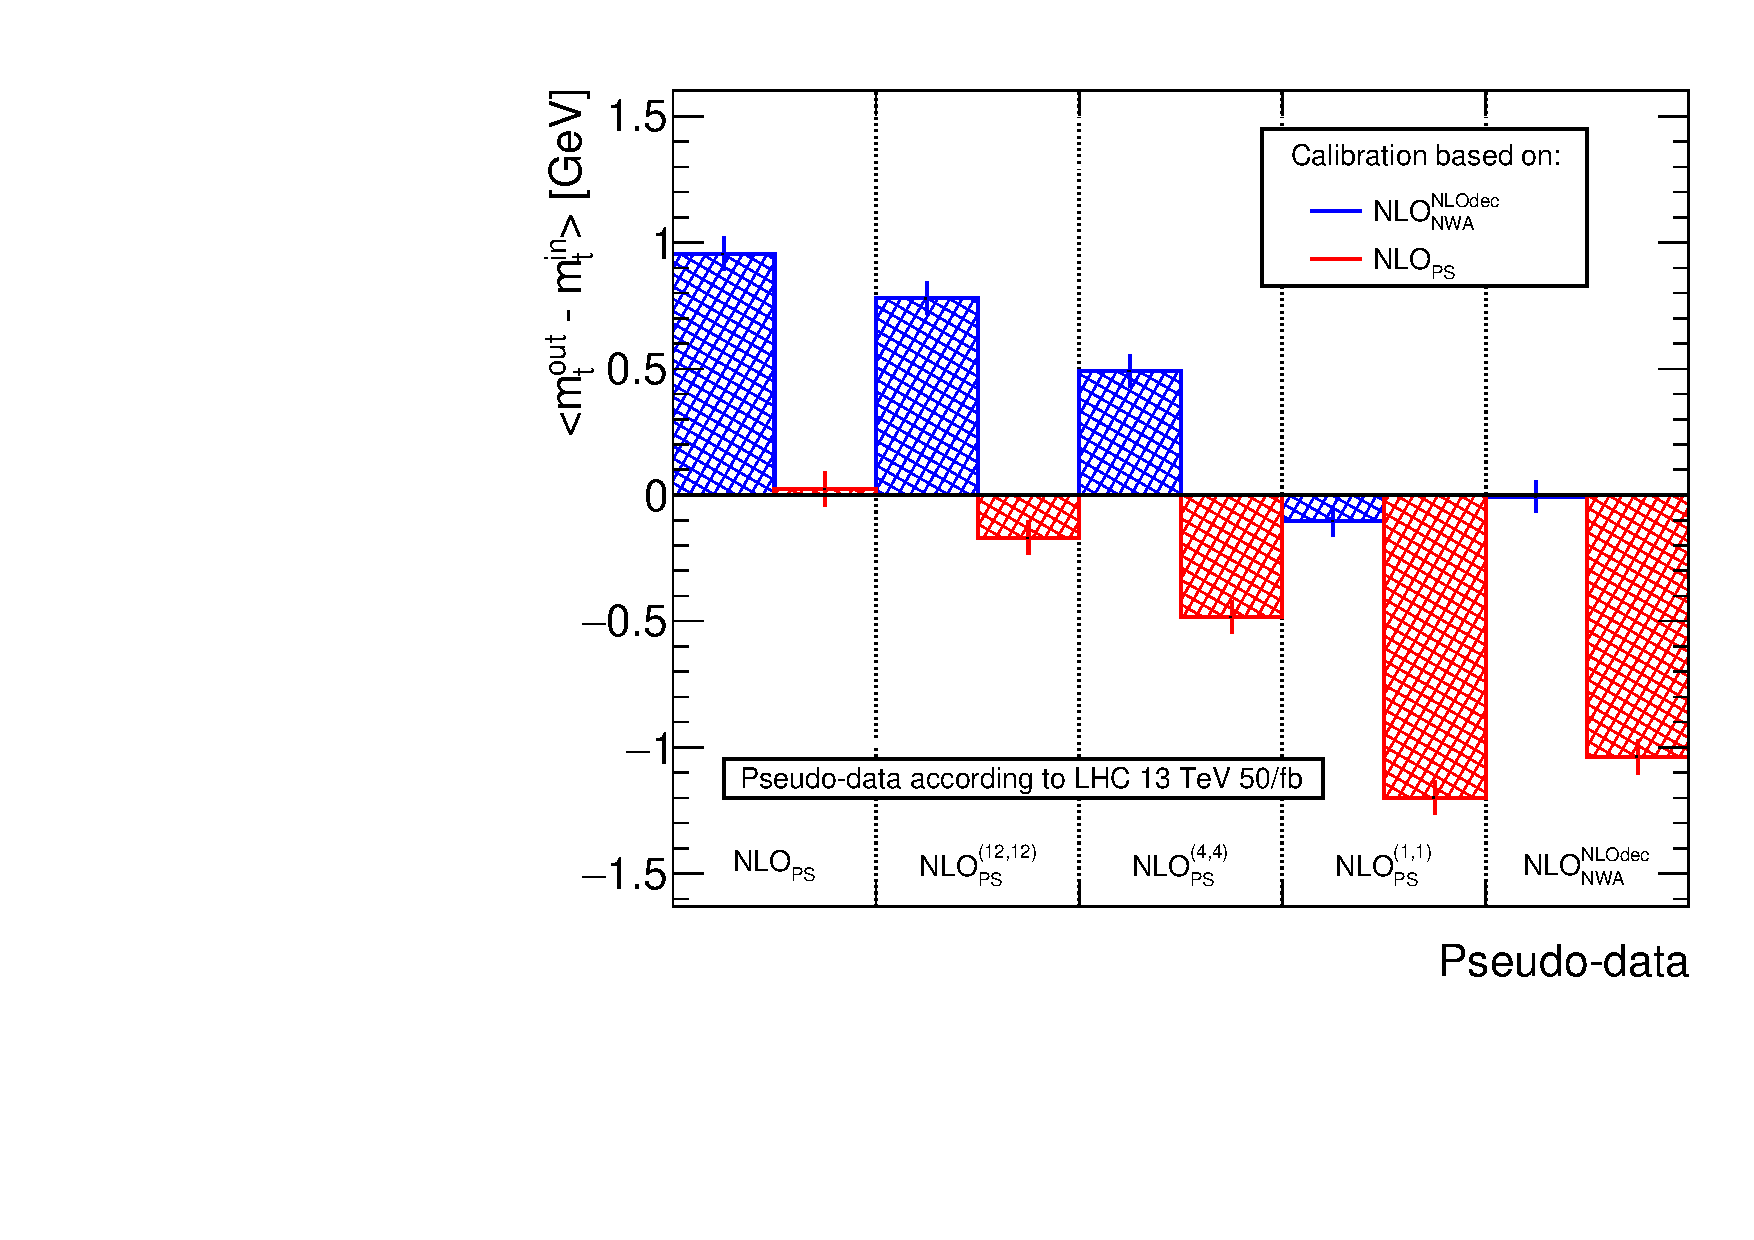
\includegraphics[width=\textwidth]{{plots/mlb_f1_DecOffsets_offset_pexpseed0}.pdf}
\vspace{\TwoFigBottom em}
\caption{\label{fig:oneemit_showers_var}}
\end{subfigure}
\hfill
\begin{subfigure}{0.495\textwidth}
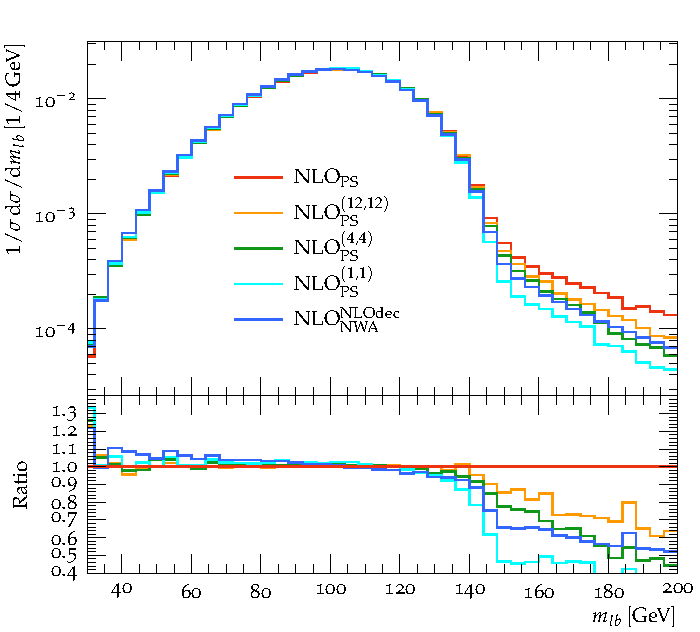
\includegraphics[width=\textwidth]{{plots/psrestricted.mlb}.pdf}
\vspace{\TwoFigBottom em}
\caption{\label{fig:oneemit_showers_var_dist}}
\end{subfigure}
\caption{\label{fig:oneemit_showers}%
  Results of the restricted-shower study for the $m_{lb}$ observable
  using $\mrm{NLO}_\mrm{PS}^{(\nprod,\ndec)}$
  parton showers that terminate after a certain maximal number of
  emissions in both the production and decay showers.
  In~(a) mass offsets are shown for a number of pseudo-data sets using
  the $\nlodec$ and the $\nlops$ calibrations in the shape analysis.
  The sets of pseudo-data are generated according to the 
  $\nlodec$ description, the default $\nlops$ as well as three $\nlops$
  showers that differ in $\nprod=\ndec=n_\mrm{max}$. The corresponding $m_{lb}$
  distributions for the case $m_t=172.5\gev$ are given in~(b).}
\end{figure}
%
\begin{figure}[t!]
\centering
\begin{subfigure}{0.495\textwidth}
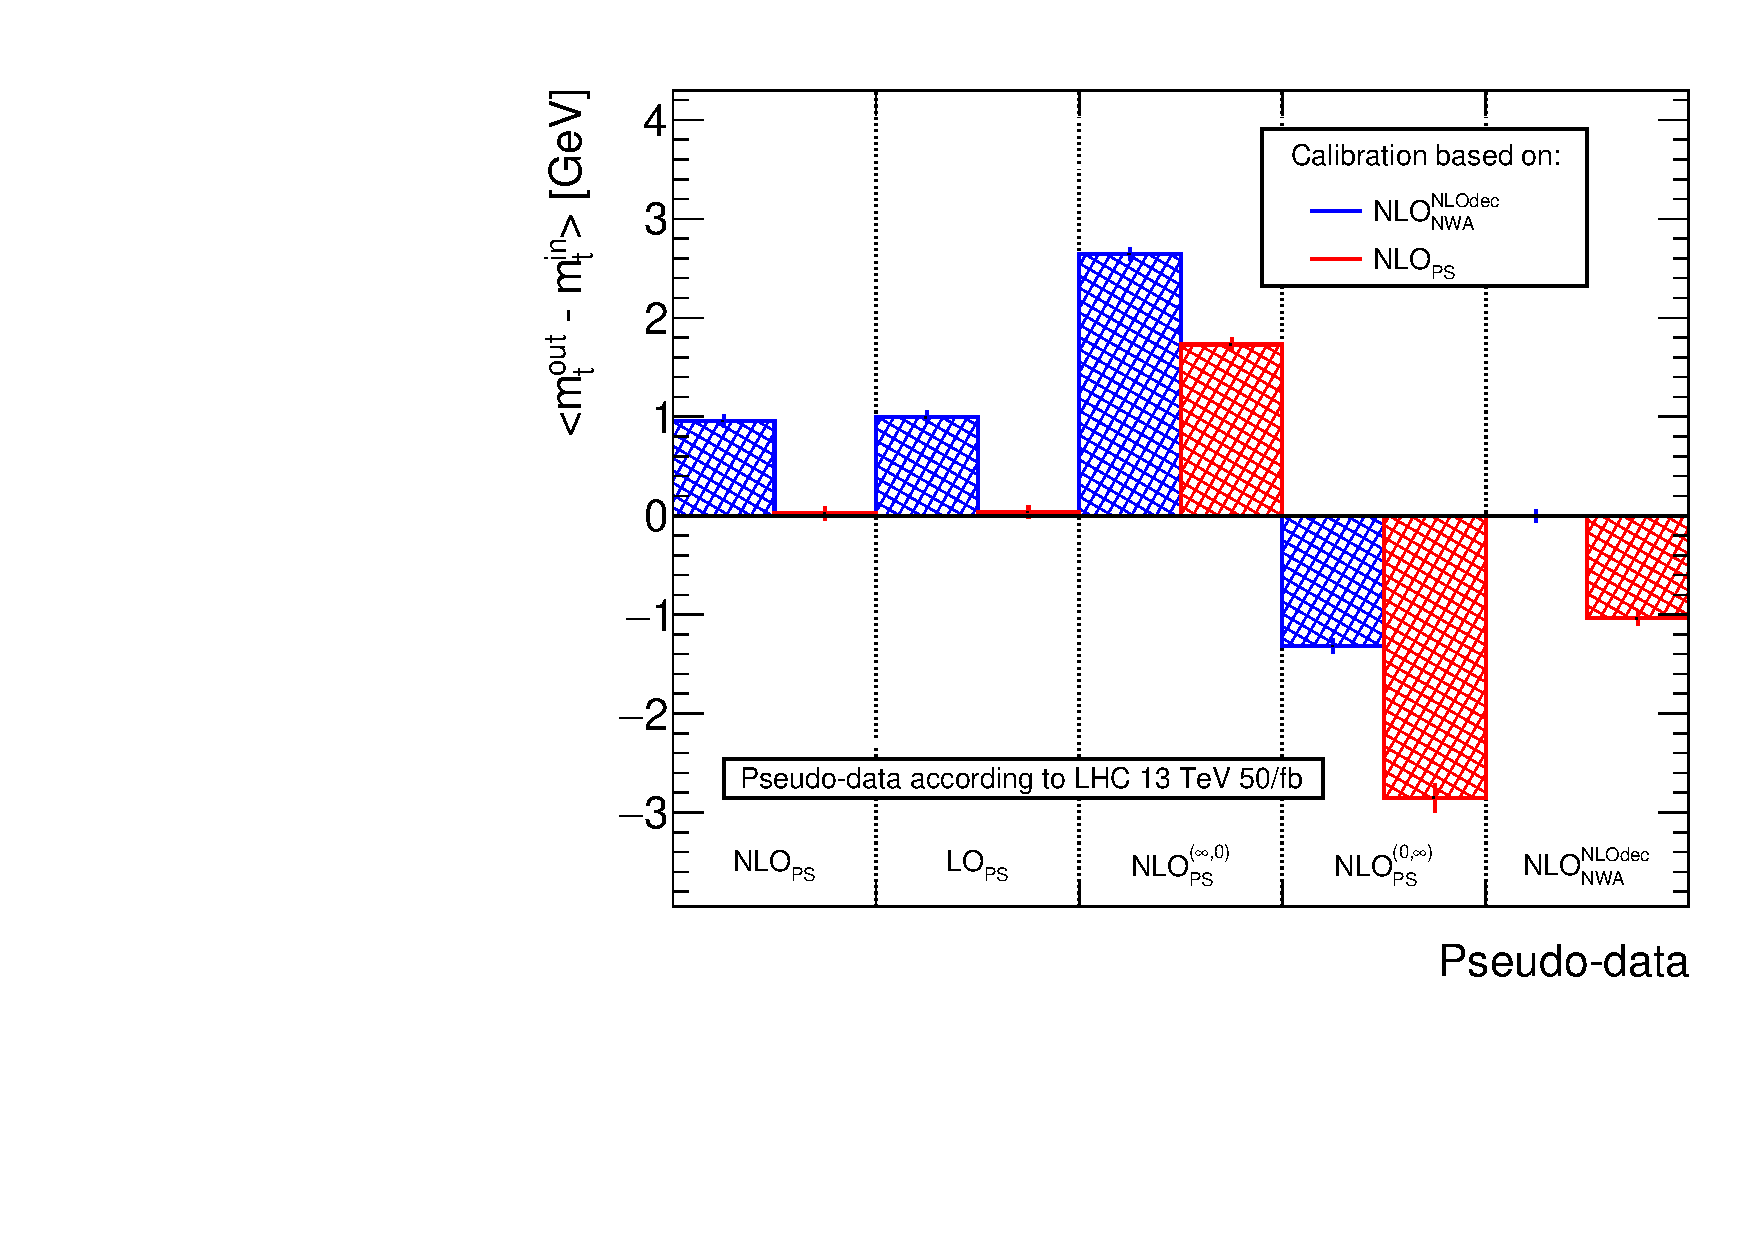
\includegraphics[width=\textwidth]{{plots/mlb_f1_DecOffsetsPure_offset_pexpseed0}.pdf}
\vspace{\TwoFigBottom em}
\caption{\label{fig:lo-prod-dec_showers_var}}
\end{subfigure}
\hfill
\begin{subfigure}{0.495\textwidth}
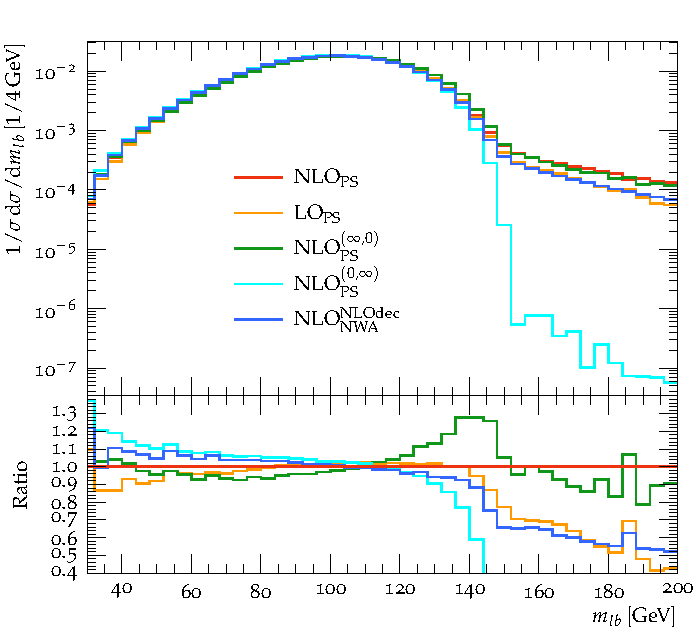
\includegraphics[width=\textwidth]{{plots/proddecay.mlb}.pdf}
\vspace{\TwoFigBottom em}
\caption{\label{fig:lo-prod-dec_showers_var_dist}}
\end{subfigure}
\caption{\label{fig:lo-prod-dec_showers}%
   Results of the restricted-shower study for the $m_{lb}$ observable
   using pure production, pure decay and pure LO parton showers only.
   In~(a) mass offsets are shown for a number of pseudo-data sets using    
   the $\nlodec$ and the $\nlops$ calibrations in the shape analysis.
   The sets of pseudo-data are generated according to the $\nlodec$
   description, the default $\nlops$ and $\lops$ showers as well as
   $\nlops$ showers whose evolution is restricted to the production or
   decay stage only. The corresponding $m_{lb}$ distributions for the
   case $m_t=172.5\gev$ are given in~(b).}
\vspace*{-4mm}
\end{figure}

\afterpage{\clearpage}

Figure~\ref{fig:oneemit_showers} summarises the results of the
restricted-shower studies.
%
 Figure~\ref{fig:oneemit_showers_var} shows the offsets and their
 statistical uncertainties for sets of pseudo-data analysed with two
 calibrations, namely $\nlops$ and $\nlodec$, while the figure to the
 right, Fig.~\ref{fig:oneemit_showers_var_dist}, depicts the
 corresponding \mlb\ distributions.
%
 The leftmost bin in Fig.~\ref{fig:oneemit_showers_var} corresponds to the
 mass shifts displayed in Fig.~\ref{fig:PS_vs_ttbar_NLO_nlodc}. The blue bar depicts the
 offset of the $\nlops$ pseudo-data, analysed with the $\nlodec$ calibration.
 The almost vanishing red bar shows the closure for the $\nlops$ pseudo-data and
 calibration.
%
 Moving to the right, the parton shower is more and more restricted,
 allowing for at
 most $12$, $4$ and $1$ emissions in each subshower.
%
 This results in a smooth transition from the offset of
 $0.96\pm0.07\gev$ to almost
 zero (with an indication of a small overshoot to negative offsets).
%
 The mass shifts becoming fairly small for more restricted showering
 indicate that most of the differences between the $\nlodec$ and
 $\nlops$ predictions emerge from resummation effects.
%
 Finally, the rightmost bin is for the $\nlodec$ pseudo-data themselves.

 The calculated offsets, obtained from fits to the \mlb\ distributions
 like the ones in Fig.~\ref{fig:oneemit_showers_var_dist},
 receive contributions from regions with large differential cross
 sections and small differences between restricted shower and
 calibration ($\nlodec$ and $\nlops$) results, as well as from regions
 with small differential cross sections and relatively large differences.
%
 The interplay of these effects can lead to situations such as the one
 observed here, where the mass offsets obtained from
 $\mrm{NLO}_\mrm{PS}^{(1,1)}$ pseudo-data are closer to the ones
 obtained by using $\nlodec$ pseudo-data, despite the fact that the
 $\mrm{NLO}_\mrm{PS}^{(4,4)}$ curve is closer to $\nlodec$ for \mlb\
 values around the kinematic edge and beyond.


We complete the parton shower studies by presenting offsets and
\mlb distributions for parton shower descriptions where we separately
switch off ($a$)~the NLO corrections to the $t\bar t$ production i.e.~use $\lops$,
($b$)~the emissions in the decay showers, denoted by~$\mrm{NLO}_\mrm{PS}^{(\infty,0)}$,
and ($c$)~the emissions in the production shower, denoted by $\mrm{NLO}_\mrm{PS}^{(0,\infty)}$.
%
For the corresponding results in Fig.~\ref{fig:lo-prod-dec_showers},
the same calibrations as in Fig.~\ref{fig:oneemit_showers} are used.
%
We find that the offsets for the $\lops$ and $\nlops$ predictions
agree very well, although the shape of the $\lops$ \mlb\ distribution
in Fig.~\ref{fig:lo-prod-dec_showers_var_dist} substantially deviates
from the $\nlops$ one outside the range $70\gev<\mlb<140\gev$.
%
This means we observe similar compensating effects in the fit as
discussed for Fig.~\ref{fig:oneemit_showers}.
%
The small difference in the offsets indicates that the NLO treatment
of the production process included by the $\nlops$ prescription has a
minor impact on the fit. The nearly vanishing offset between
the $\lops$ pseudo-data and $\nlops$ calibration is likely to be a consequence of
the same resummation corrections being applied in both showers.

%
The $\mrm{NLO}_\mrm{PS}^{(\infty,0)}$ prediction in Fig.~\ref{fig:lo-prod-dec_showers}
can be considered as the shower correction to $t\bar t$ production at NLO ($\lodec$), 
while the $\mrm{NLO}_\mrm{PS}^{(0,\infty)}$ prediction represents the shower approximation to the
radiative corrections in the top quark decays.
%
The use of the related pseudo-data increases the absolute mass offsets
for both the $\nlops$ and the $\nlodec$ calibration, illustrating that
the production shower predominantly evolves through initial-state
radiation (resulting in larger fitted \mt) while the decay showers are
mostly driven by final-state radiation (yielding smaller \mt).
%
This is induced by the corresponding \mlb\ distributions in
Fig.~\ref{fig:lo-prod-dec_showers_var_dist}, where we observe that the
$\mrm{NLO}_\mrm{PS}^{(\infty,0)}$ prediction is enhanced for larger \mlb
values, in particular around the kinematic edge of the distribution,
while the $\mrm{NLO}_\mrm{PS}^{(0,\infty)}$ prediction turns out to be
softer than the others, showing a very sharp kinematic edge.
%
For the $\nlodec$ calibration, the sum of the mass
offsets for production shower pseudo-data, amounting to
$2.65\pm0.07\gev$, and decay showers pseudo-data, amounting to
$-1.32\pm0.07\gev$, is close to the mass shift of $0.96\pm0.07\gev$
obtained for $\nlops$ pseudo-data.
%
This means that the generation-level factorisation (dissection) of the emission
patterns for production and decays almost completely carries over to
the analysis level.

\begin{figure}[tbp!]
  \centering
  \begin{subfigure}{0.495\textwidth}
    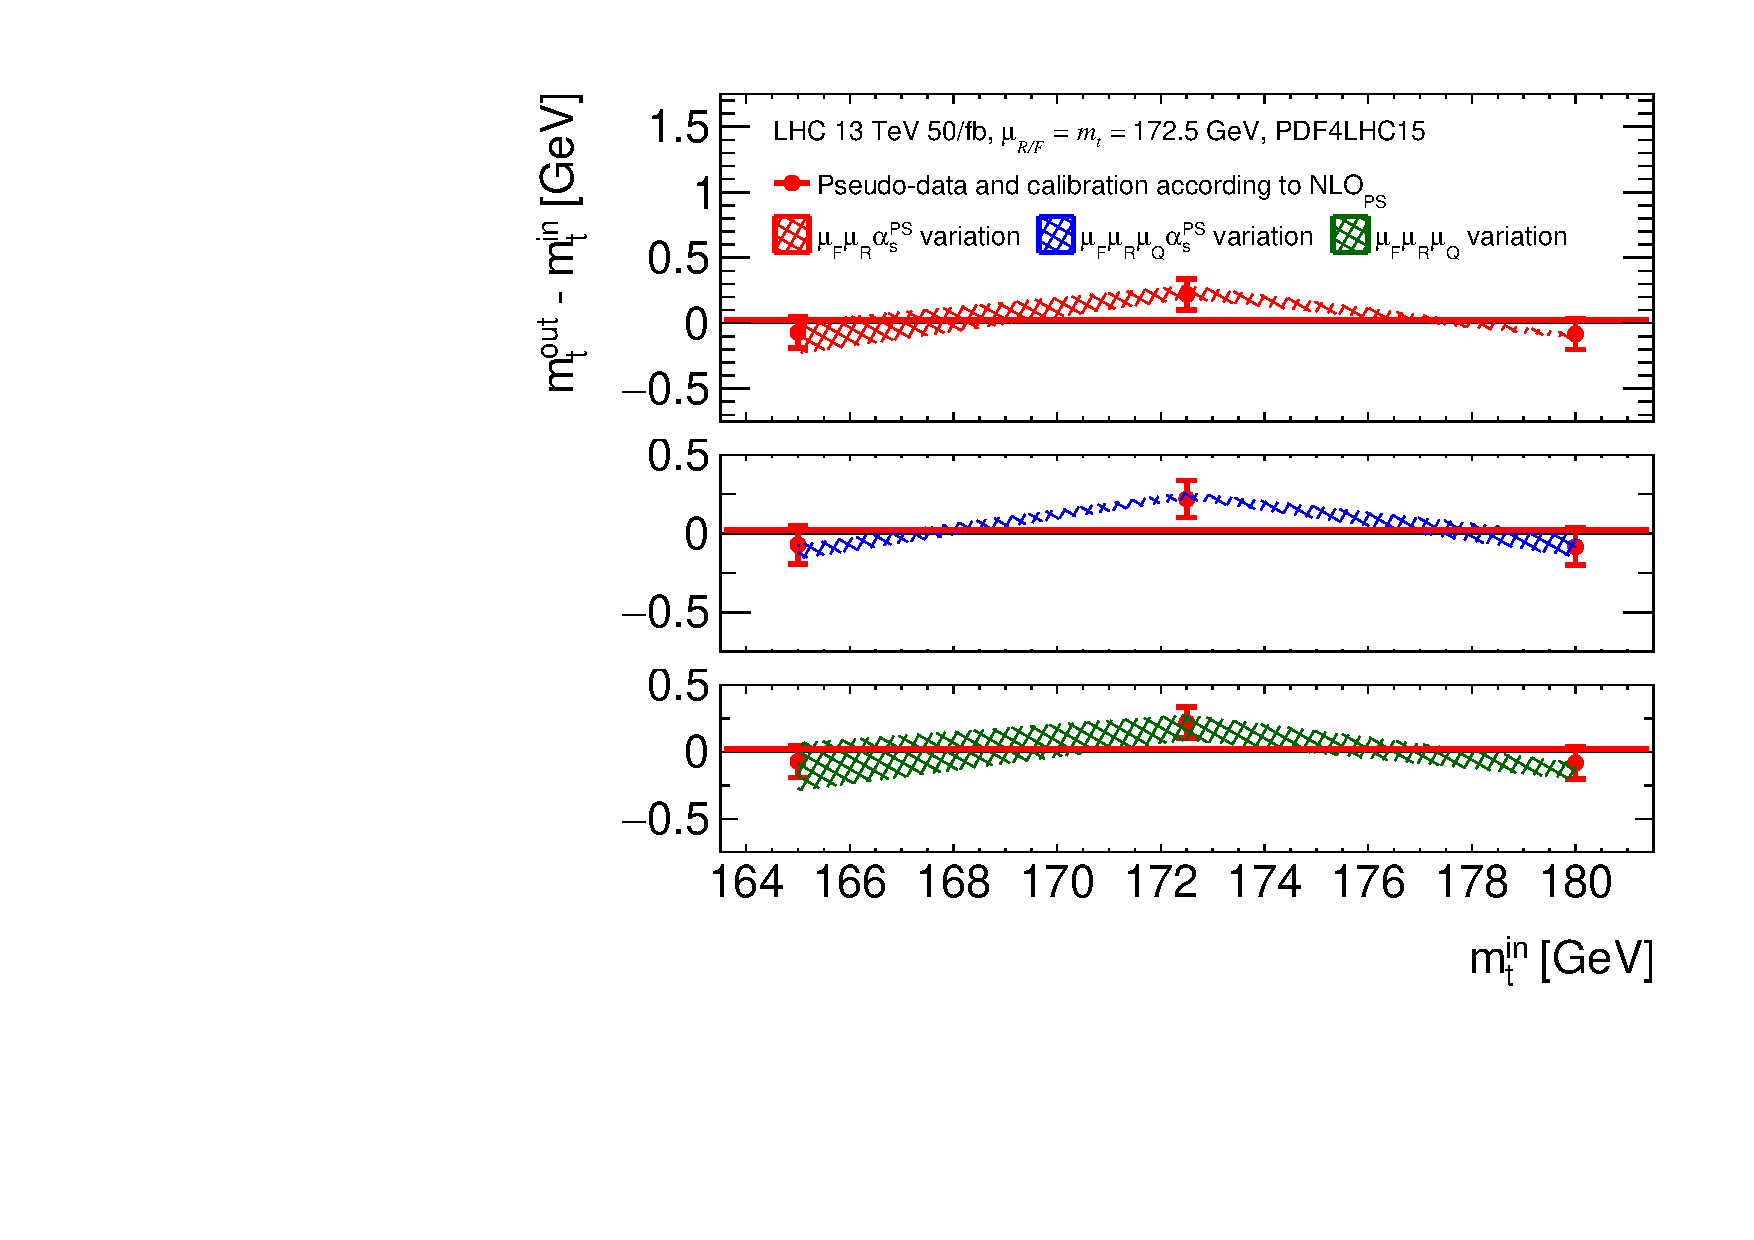
\includegraphics[width=\textwidth]{{plots/mlb_f1_PSvars_NLO_pexpseed0}.pdf}
    \caption{\label{fig:PS_scale_var}}
  \end{subfigure}
  \hfill
  \begin{subfigure}{0.495\textwidth}
    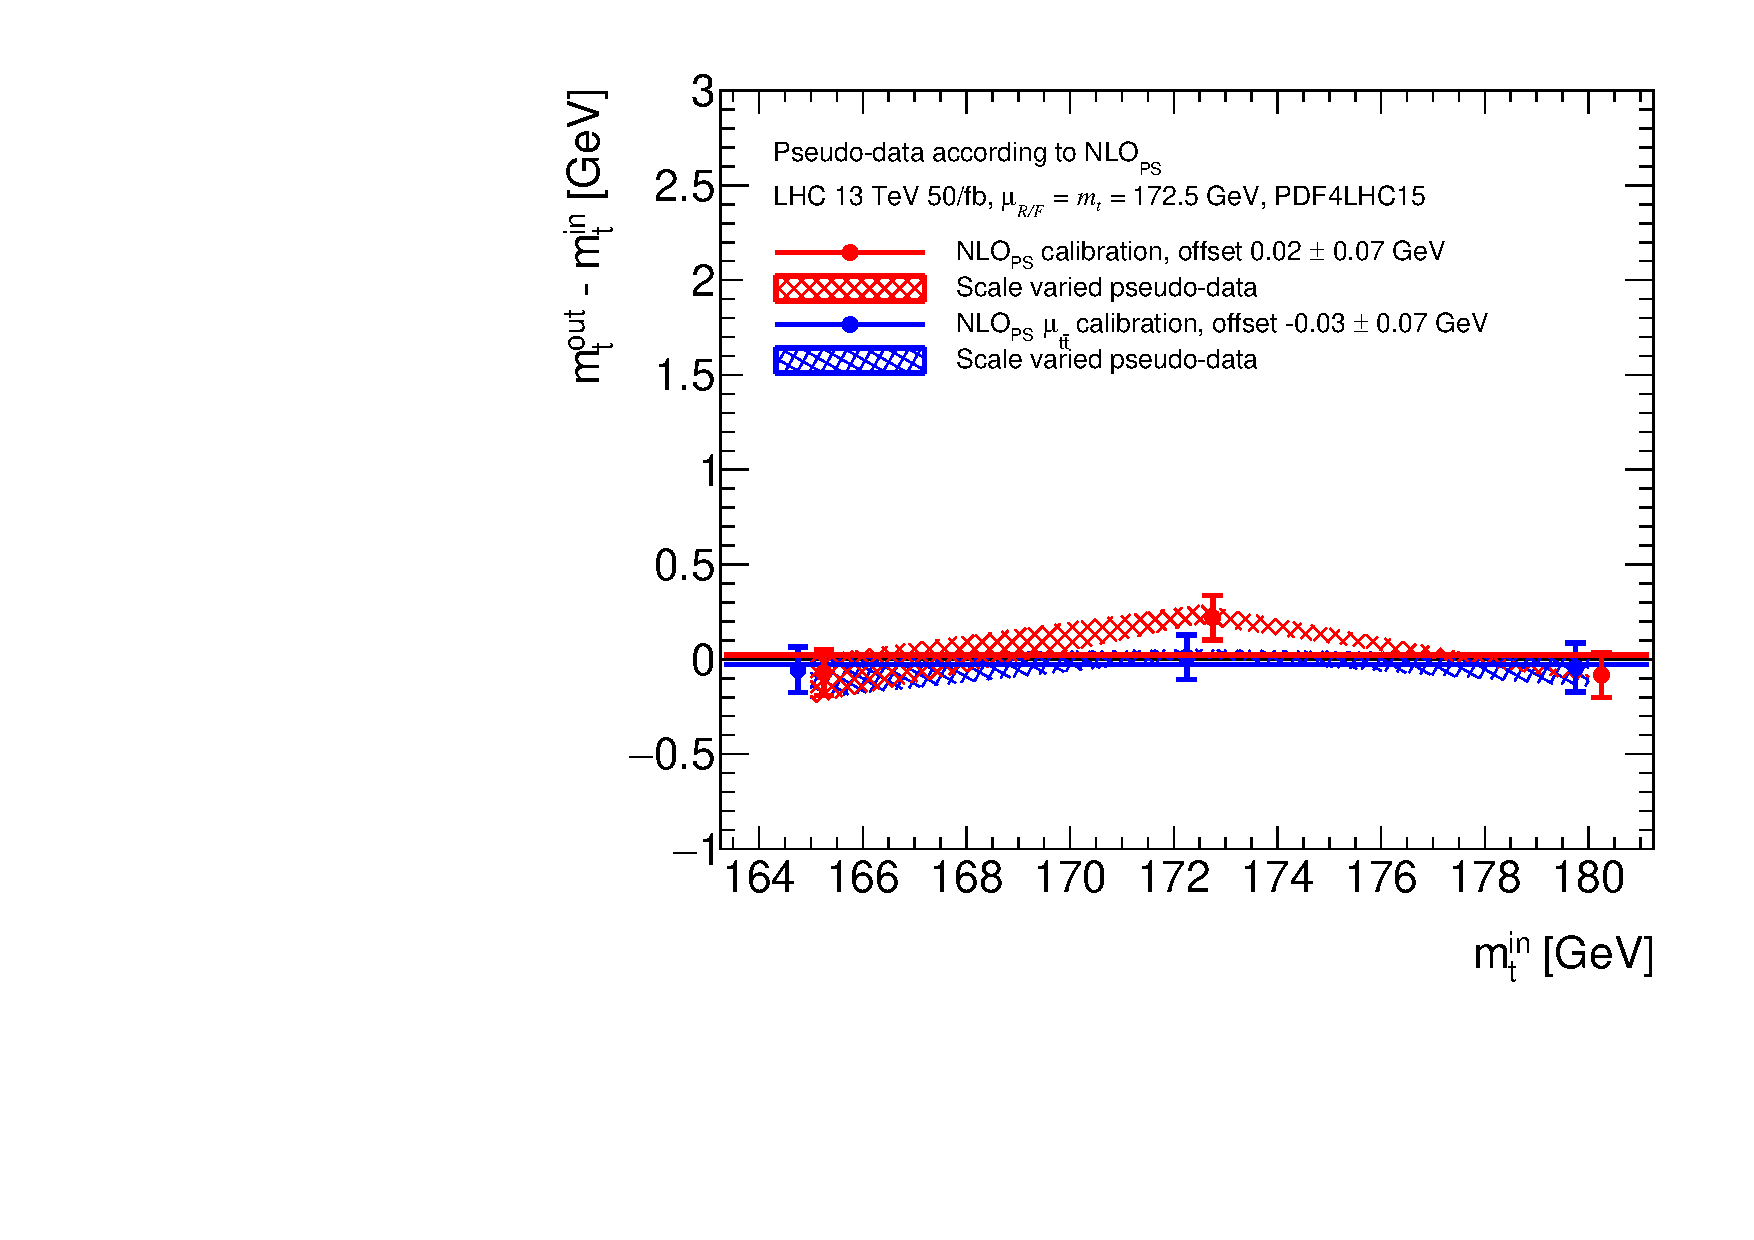
\includegraphics[width=\textwidth]{{plots/mlb_f1_13TeVstd_PS_scale_NLO_pexpseed0}.pdf}
    \caption{\label{fig:PS_scale_NLO}}
  \end{subfigure}
  \caption{\label{fig:PS_scale}%
    Results for different schemes determining the parton shower scale
    dependence using the $m_{lb}$ observable and pseudo-data as well
    as calibrations derived from $\nlops$ predictions.
    In~(a), the uncertainty bands are shown for the different ways of
    evaluating the shower scale dependence (cf.~Section~\ref{subsec:input}).
    The offsets and uncertainty bands for different central scale
    choices used in the computation of the hard process are shown in~(b).}
\end{figure}

The \mlb distributions of the restricted and full showering show clear
differences. To quantify the significance of these differences, the
parton shower scale uncertainties are assessed.
%
For the decay showers, we performed a decay shower starting scale variation by
using factors of $0.5$ and $2.0$ applied to the central scale $\muqdec$. Despite this wide range for varying the resummation scales, we find negligible differences in the shapes of the \mlb\ distributions.
%
Therefore, all variations of the shower description employed here are always based on the fixed value $\muqdec=M_W/2$.
%
We use the different schemes described in Section~\ref{subsec:input}
to obtain the scale-variation induced theory uncertainties of the $\nlops$
prescription presented in Fig.~\ref{fig:PS_scale_var}.
%
While the combined variation, $\mu_F\mu_R\mu_Q\as{\mathrm{PS}}$, leads to the smallest uncertainty band, the band based on the $\mu_F\mu_R\mu_Q$ parameter variation is marginally larger.
%
Most notably, these differences are much smaller than those occurring between
the various theory descriptions discussed above.

Finally, for the $\nlops$ calculations, we compare in Fig.~\ref{fig:PS_scale_NLO}  
the results for the two central-scale choices $\mu_R=\mu_F=m_t$ and $\mu_R=\mu_F=\mu_{t\bar t}$ as defined in Eq.~(\ref{eq:scale_ttb}).
%
Although the predicted total cross sections listed in the last two rows of Table~\ref{tab:xs} depend on this choice, the two predictions lead to consistent measured top quark masses, i.e.~the associated offsets agree within their uncertainties.

As can be inferred from Fig.~\ref{fig:massvar_fullNLO_mlb}, the sensitivity of
the \mlb\ observable to the top quark mass, and consequently the achievable
statistical uncertainty on \mt\ in data, depends on the fit range used.
%
In this context, the range $140$--$160\gev$ is a particularly \mt-sensitive
region, which however also features sizeable differences in the theoretical
descriptions, for example as shown in Fig.~\ref{fig:scalevar_mlb}.
%
Consequently, the resulting offsets listed in Table~\ref{tab:offset}
depend on the chosen fit range.
%
As an example, restricting the fit to $\mlb<140\gev$ results in
differences in the offsets of the order of $0.1$--$0.4\gev$, where in
general larger differences are observed for larger absolute offsets.
%
An experimental analysis should be optimised for the smallest total
uncertainty, including the variation of the relative importance of statistical
and systematic uncertainties, while changing the fit range. Therefore we
consider the results shown in Table~\ref{tab:offset}, based on the fit ranges
given in Eq.~(\ref{eq:fitranges}), as our nominal values.


%--------------------------------------------------------------------------
\begin{table}[tb!]
\small
\begin{center}
\begin{tabular}{|l|l|c|c|c|c|c|}
\cline{3-6}
\multicolumn{2}{c}{}         & \multicolumn{2}{|c|}{Offset [GeV]} &
\multicolumn{2}{|c|}{Figure} & \multicolumn{1}{c}{}\\\hline
 Pseudo-data &  Calibration & \mlb & \mtwo  &\mlb & \mtwo & \Chiq \\\hline
\hline
&&&&&&\\
 $\lodec$  & $\mathrm{LO_{NWA}^{LOdec}}$ & $+0.51 \pm 0.06$ &$+0.48 \pm 0.04$ &
 \ref{fig:LOvsNLO_NWA_decayLO} & \ref{fig:LOvsNLO_NWA_decayLO_mt2}   & 0.17\\
%
 $\nlodec$ &                 $\lodec$ & $-1.80 \pm 0.06$ &$-1.67 \pm 0.04$ &
 \ref{fig:NLO_NWA_decayLOvsNLO} & \ref{fig:NLO_NWA_decayLOvsNLO_mt2} & 3.25\\
%
 $\nlodec$ & $\mathrm{LO_{NWA}^{LOdec}}$ & $-1.38 \pm 0.07$ &$-1.24 \pm 0.05$ &
 \ref{fig:NLO_NWA_decayNLO} & \ref{fig:NLO_NWA_decayNLO_mt2}         & 2.65\\
%
$\nlofull$ &                $\lofull$ & $-1.52 \pm 0.07$ &$-1.62 \pm 0.05$ &
 \ref{fig:fullNLO} & \ref{fig:fullNLO_mt2}                           & 1.35\\
%
$\nlofull$ &                $\nlodec$ & $+0.83 \pm 0.07$ &$+0.60 \pm 0.06$ &
 \ref{fig:NLO_WWbb_vs_NWA_decayNLO} & \ref{fig:NLO_WWbb_vs_NWA_decayNLO_mt2}
                                                                     & 6.22\\
%
$\nlofull$ &                 $\nlops$ & $-0.09 \pm 0.07$ &$-0.07 \pm 0.06$ &
 \ref{fig:WWbb_vs_PS_NLO} & \ref{fig:WWbb_vs_PS_NLO_mt2}             & 0.05\\
%
  $\nlops$ &                 $\lodec$ & $-0.92 \pm 0.07$ &$-1.17 \pm 0.05$ &
\ref{fig:PS_vs_ttbar_NLO} & \ref{fig:PS_vs_ttbar_NLO_mt2}            & 8.45 \\
%
  $\nlops$ &                $\nlodec$ & $+0.96 \pm 0.07$ &$+0.68 \pm 0.05$ &
\ref{fig:PS_vs_ttbar_NLO_nlodc} & \ref{fig:PS_vs_ttbar_NLO_nlodc_mt2}& 10.59\\
%\
  $\nlops$ &   $\nlops~(\mu_{t\bar{t}})$ & $-0.03 \pm 0.07$ &$+0.02 \pm 0.05$ &
 \ref{fig:PS_scale_NLO} & \ref{fig:PS_scale_NLO_mt2}                 & 0.34\\
%
&&&&&&\\
\hline
\end{tabular}
\end{center}
\caption{Summary of the offsets observed when analysing pseudo-data listed in
  the first column with template fit functions calibrated based on various
  theoretical predictions as given in the second column.
%
 The observed offsets for the two observables \mlb\ and \mtwo\ are reported in
 the second pair of columns, where the corresponding figures are listed in the
 next pair of columns.
%
 Finally, the \Chiq\ for the differences in the offsets for the two observables
 are displayed in the rightmost column, see text for further details.
%
\label{tab:offset}}
\end{table}
%--------------------------------------------------------------------------


\boldmath
\subsection{Fit results for $\mtwo$}
\unboldmath


The investigations performed for the \mlb\ observable are repeated for \mtwo.
%
 The results corresponding to Figs.~\ref{fig:LOvsNLO_NWA_decayLO}
 to~\ref{fig:PS_scale_NLO} are shown in Figs.~\ref{fig:LOvsNLO_NWA_decayLO_mt2}
 to~\ref{fig:PS_scale_NLO_mt2}.
%
 Also for \mtwo, the offsets obtained when using the corresponding pair of
 pseudo-data and calibration are consistent with zero, i.e.~the method is
 closed.


 While most observations are consistent for the \mlb\ and \mtwo\ observables,
 there are some remarkable differences.
%
 For \mtwo, comparing distributions with LO and NLO in production generally results in
 an \mt\-dependent offset. 
This indicates that the NLO prediction has a weaker mass dependence
than the LO one.
%
 The slope of the \mlb\ distribution in
 Fig.~\ref{fig:NLO_PS_vs} is less steep than the one in Fig.~\ref{fig:NLO_PS_vs_mt2}. This indicates a
 different effect of the parton shower
 on the more inclusive \mtwo, retaining a higher sensitivity to the
 top quark mass.


 The offsets observed for the various pairs of pseudo-data and calibration are
 given in Table~\ref{tab:offset}.
%
 The comparison of the offsets obtained for \mtwo\ with those for \mlb\
 exhibits a very similar pattern.
 To investigate whether the sensitivity of the observables to differences in the
 theoretical predictions coincides, the differences in their offsets are
 expressed by a \Chiq\ calculated from the offsets, using the fact that the
 offsets are uncorrelated for their statistical uncertainties.\footnote{Given
   $\Oi{o}{i}\pm \Oi{u}{i}$ for the offsets \Oi{o}{i}\ and their uncertainties
   \Oi{u}{i}\ with $i=1,2=\mlb, \mtwo$, the \Chiq\ is defined as:
   $\Chiq=(\Oi{o}{1}-\Oi{o}{2})^2/ (\Oi{u}{1}^2+\Oi{u}{2}^2)$.}
For a number of pairs the differences of the offsets for \mlb\ and \mtwo\ are
 consistent with zero, leading to small values of \Chiq,
for example when comparing $\lodec$ with $\mathrm{LO_{NWA}^{LOdec}}$
 (Figs.~\ref{fig:LOvsNLO_NWA_decayLO} and
 \ref{fig:LOvsNLO_NWA_decayLO_mt2}).
%
  In contrast, most notably for the pair $\nlops$ and $\nlodec$
(Figs.~\ref{fig:PS_vs_ttbar_NLO_nlodc} and \ref{fig:PS_vs_ttbar_NLO_nlodc_mt2}),
  the difference is significant, leading to a large \Chiq.
%
 This means, at the expected statistical precision of the $13\tev$ LHC, the two
 estimators exhibit different sensitivities to this difference in the
 theoretical prediction.

\begin{figure}[tbp!]
\centering
\begin{subfigure}{0.495\textwidth}
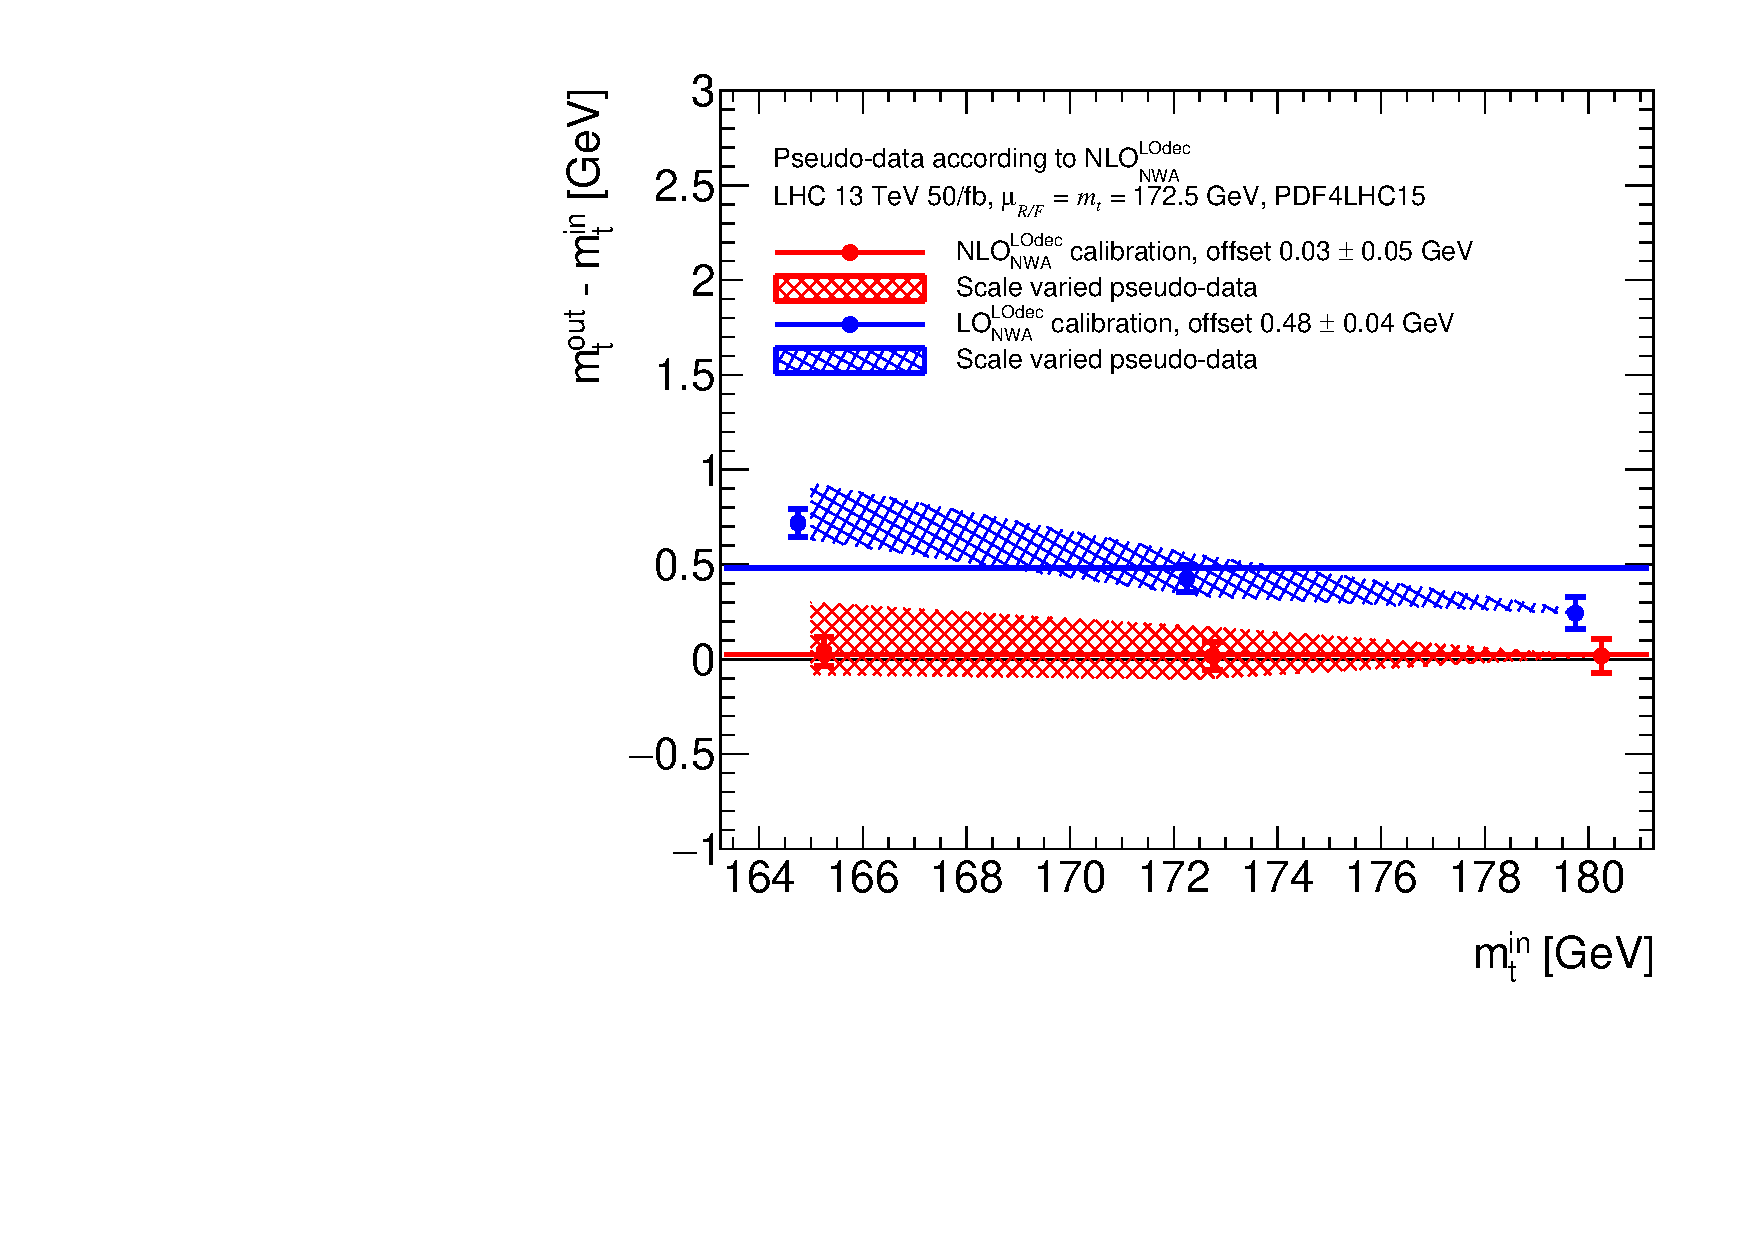
\includegraphics[width=\textwidth]{{plots/mt2_f1_13TeVstd_NLO_vs_LO_pexpseed0}.pdf}
\vspace{\TwoFigBottom em}
\caption{\label{fig:LOvsNLO_NWA_decayLO_mt2}}
\end{subfigure}
\hfill
\begin{subfigure}{0.495\textwidth}
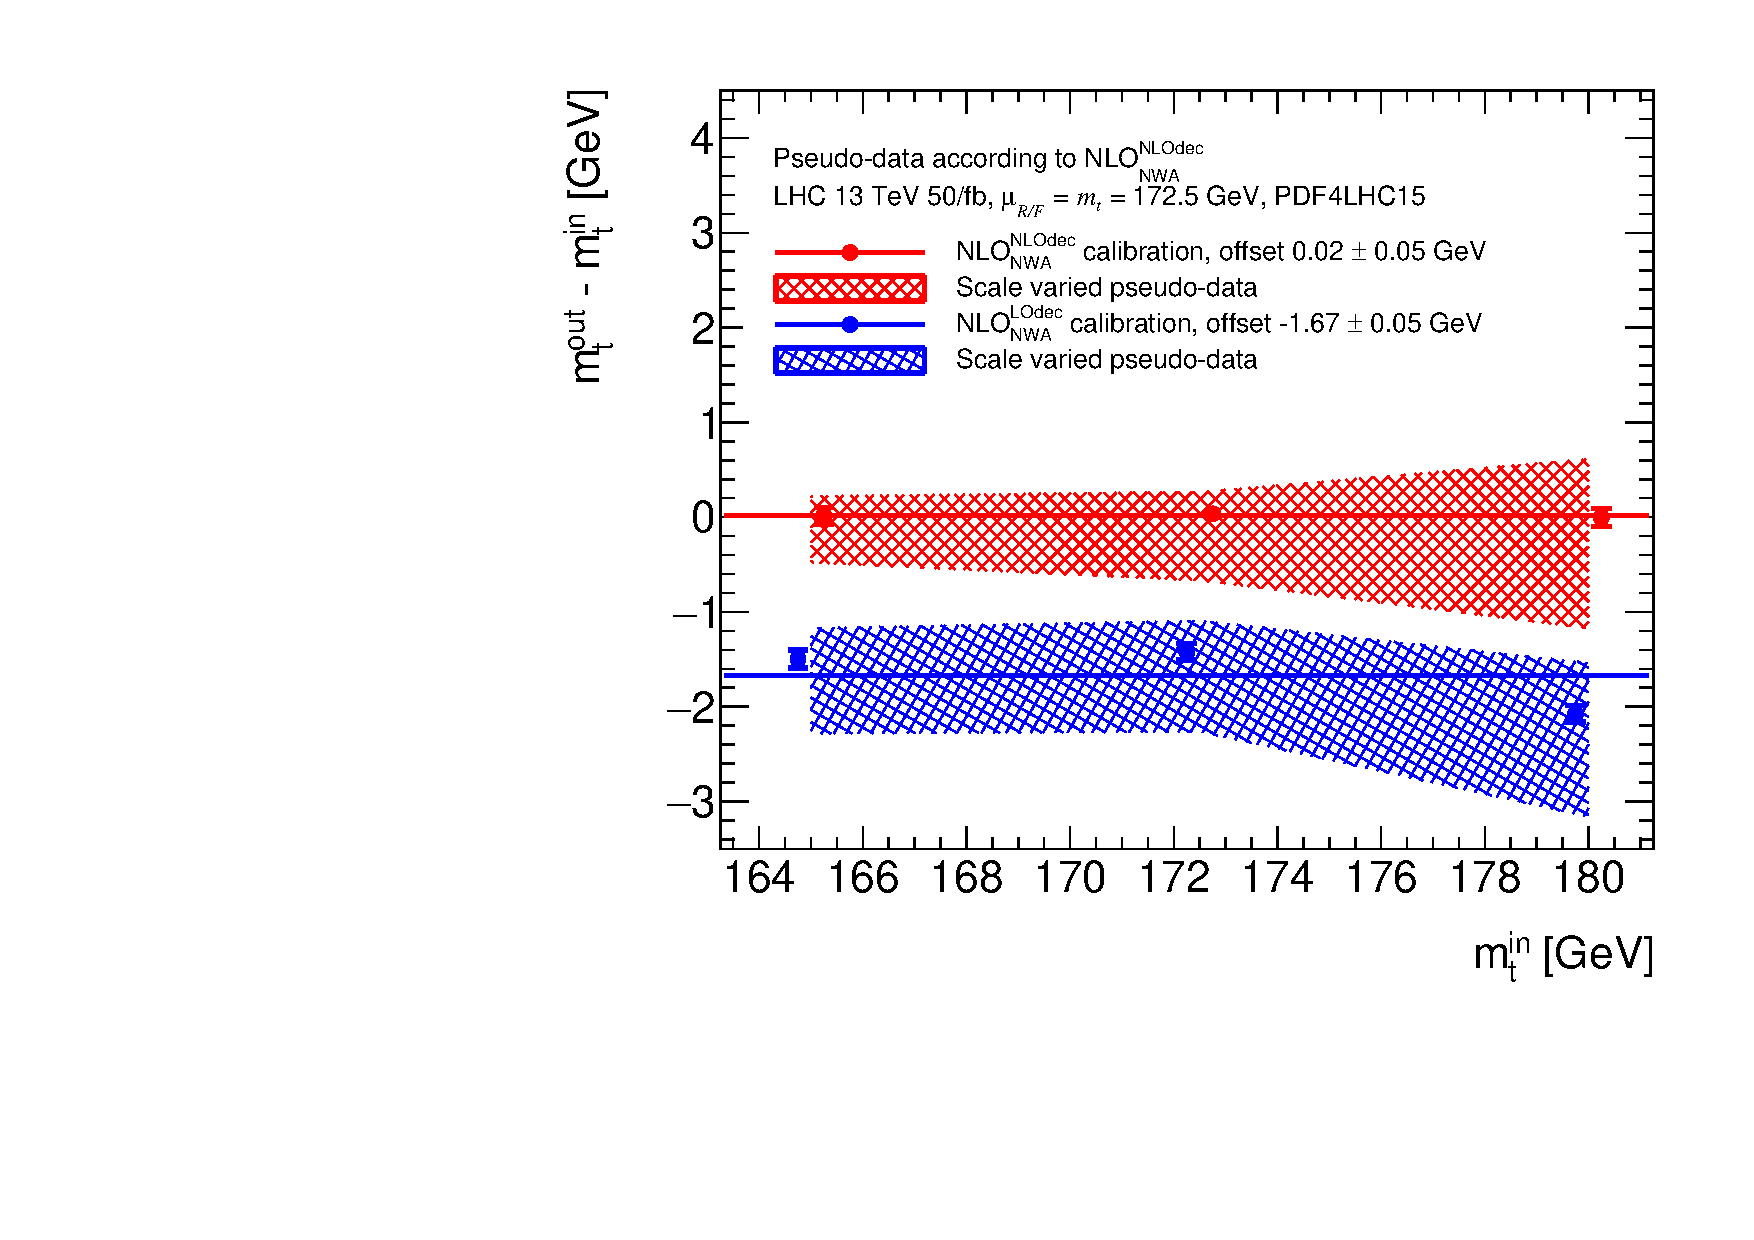
\includegraphics[width=\textwidth]{{plots/mt2_f1_13TeVstd_decay_order_pexpseed0}.pdf}
\vspace{\TwoFigBottom em}
\caption{\label{fig:NLO_NWA_decayLOvsNLO_mt2}}
\end{subfigure}
\caption{\label{fig:NWA_mt2}%
  Same as Fig.~\ref{fig:NWA} but for the observable $m_{T2}$.}
\end{figure}


\begin{figure}[tbp!]
\centering
\begin{subfigure}{0.495\textwidth}
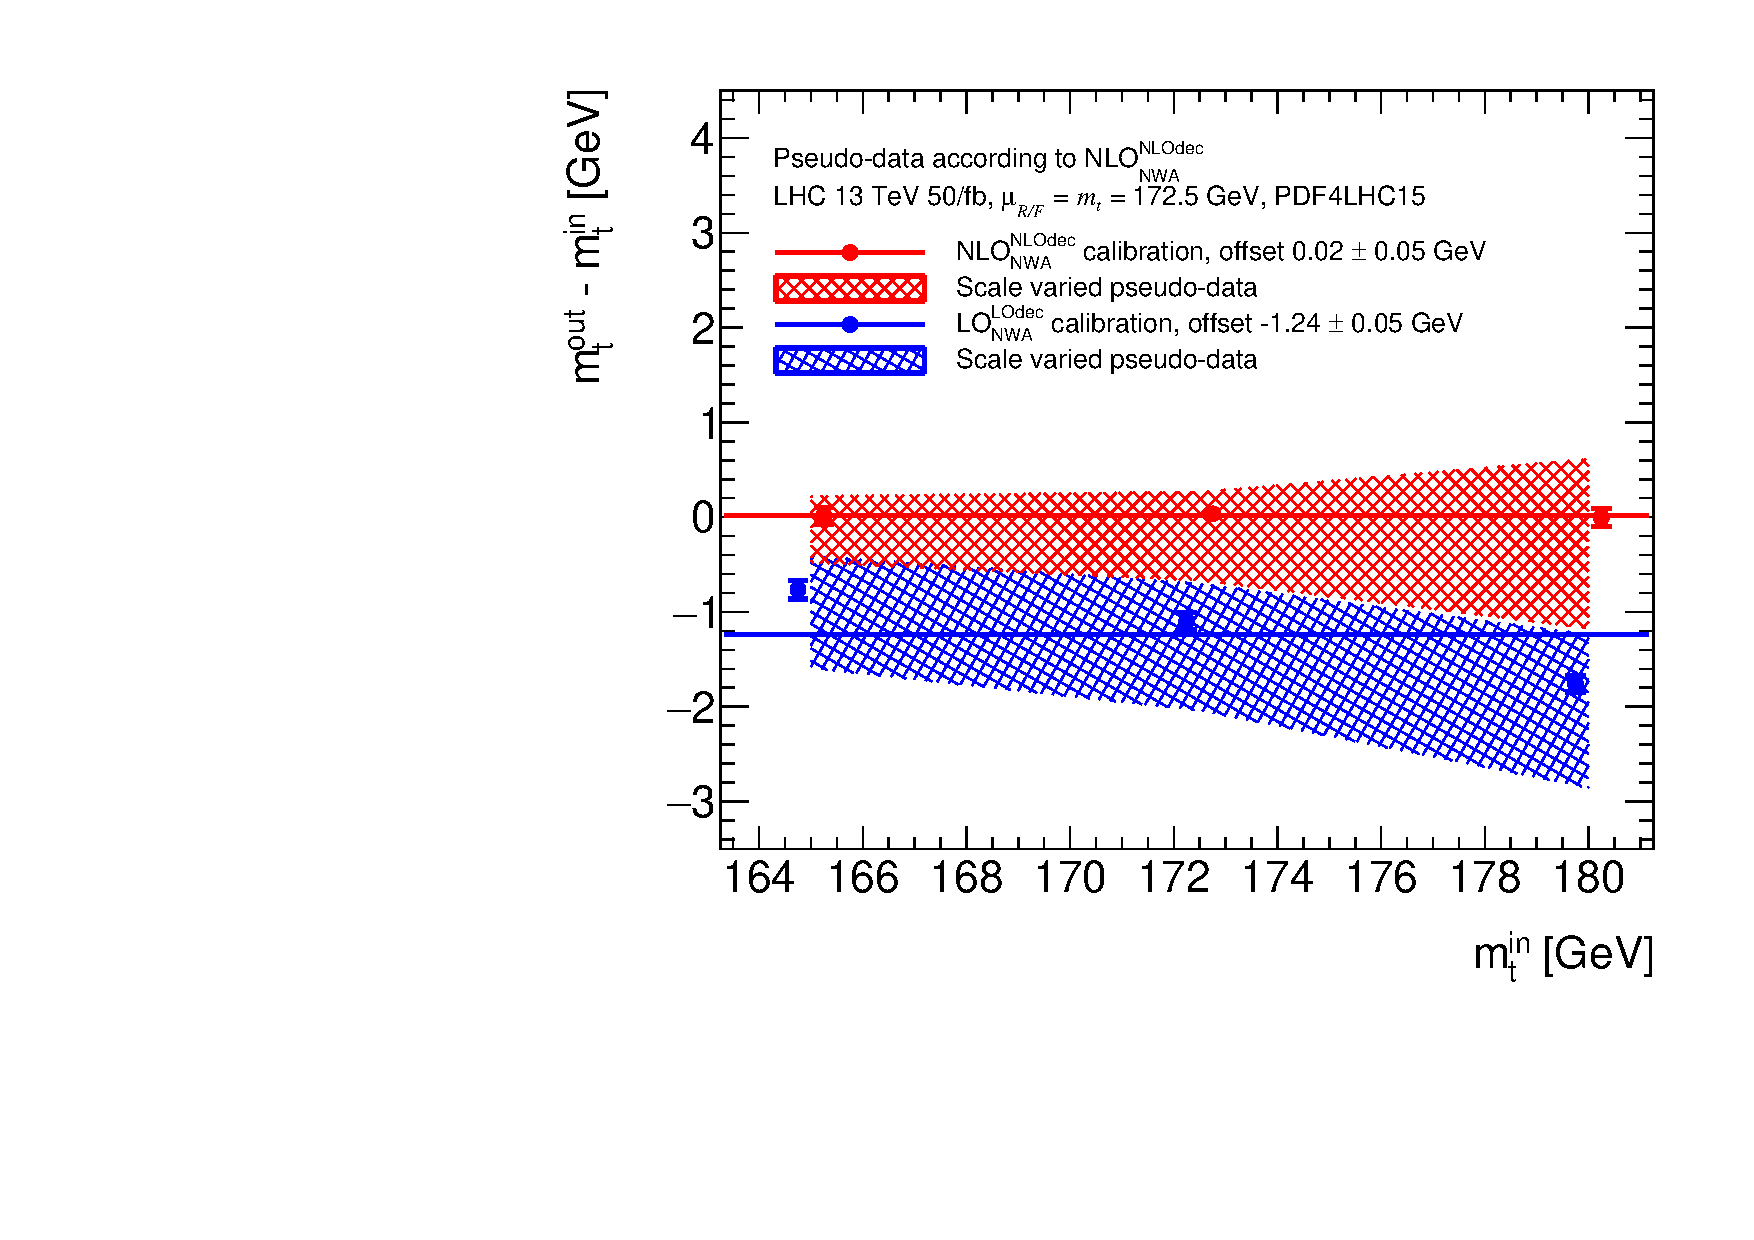
\includegraphics[width=\textwidth]{{plots/mt2_f1_13TeVstd_NLOn_vs_LO_pexpseed0}.pdf}
\vspace{\TwoFigBottom em}
\caption{\label{fig:NLO_NWA_decayNLO_mt2}}
\end{subfigure}
\hfill
\begin{subfigure}{0.495\textwidth}
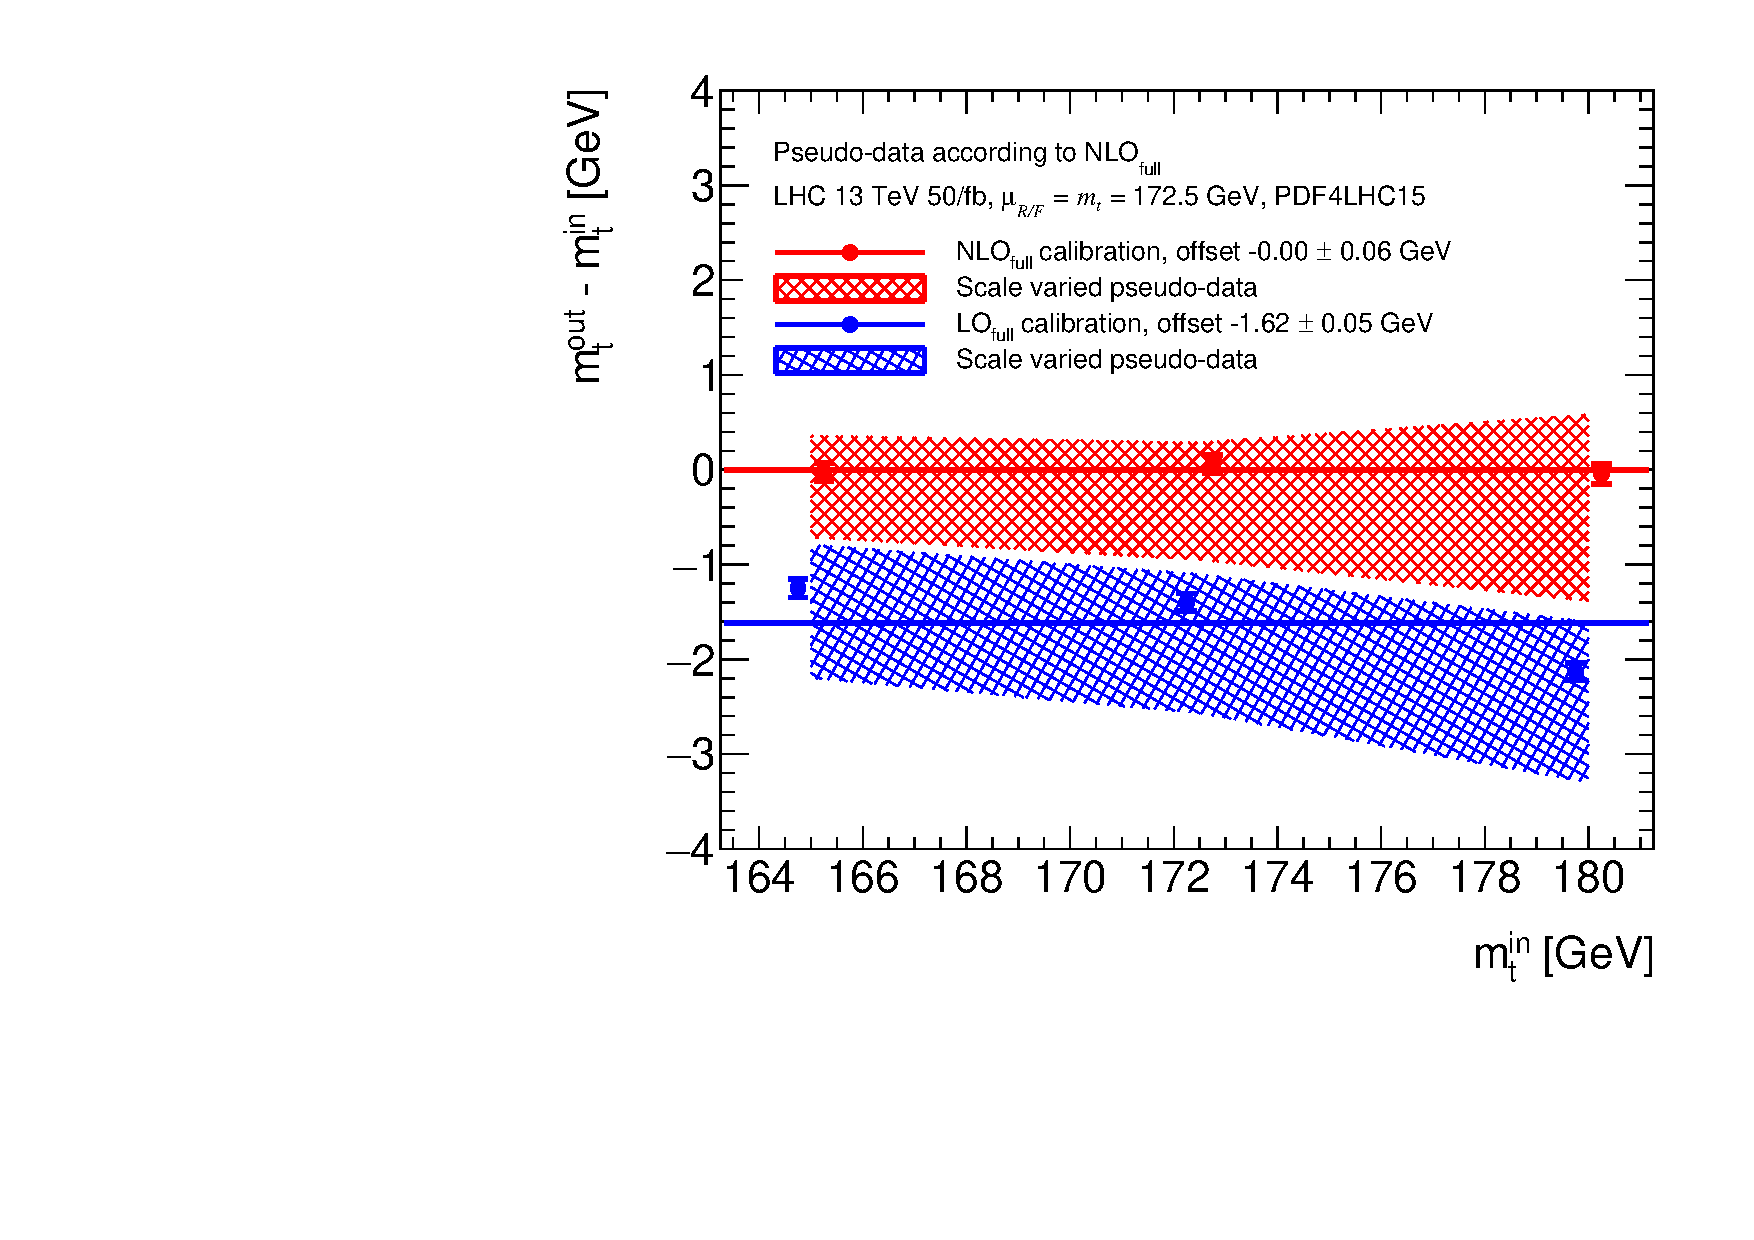
\includegraphics[width=\textwidth]{{plots/mt2_f1_13TeVstd_WWbb_diff_pexpseed0}.pdf}
\vspace{\TwoFigBottom em}
\caption{\label{fig:fullNLO_mt2}}
\end{subfigure}
\caption{\label{fig:NWAboth_mt2}%
  Same as Fig.~\ref{fig:NWAboth} but for the observable $m_{T2}$.}
\end{figure}


\begin{figure}[tbp!]
\centering
\begin{subfigure}{0.495\textwidth}
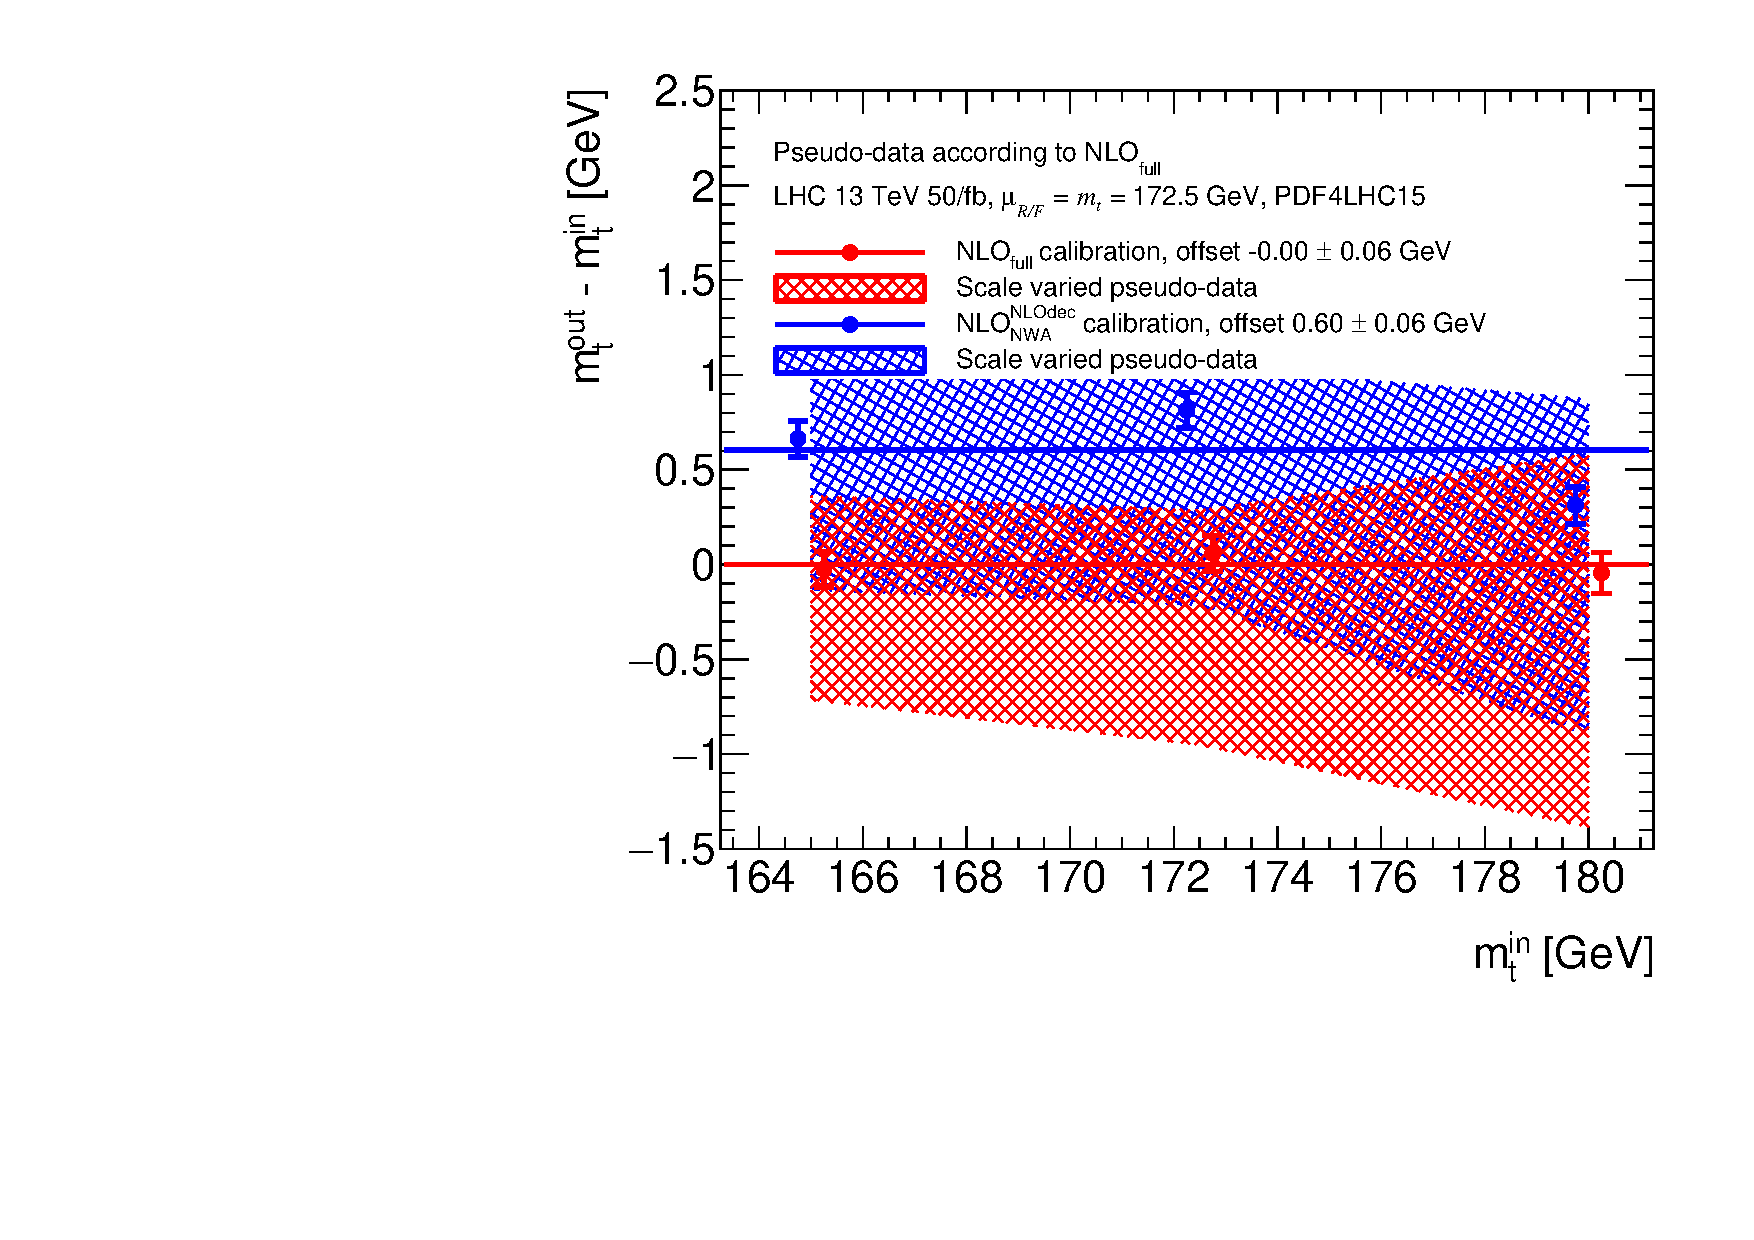
\includegraphics[width=\textwidth]{{plots/mt2_f1_13TeVstd_WWbb_vs_ttbar_pexpseed0}.pdf}
\vspace{\TwoFigBottom em}
\caption{\label{fig:NLO_WWbb_vs_NWA_decayNLO_mt2}}
\end{subfigure}
\hfill
\begin{subfigure}{0.495\textwidth}
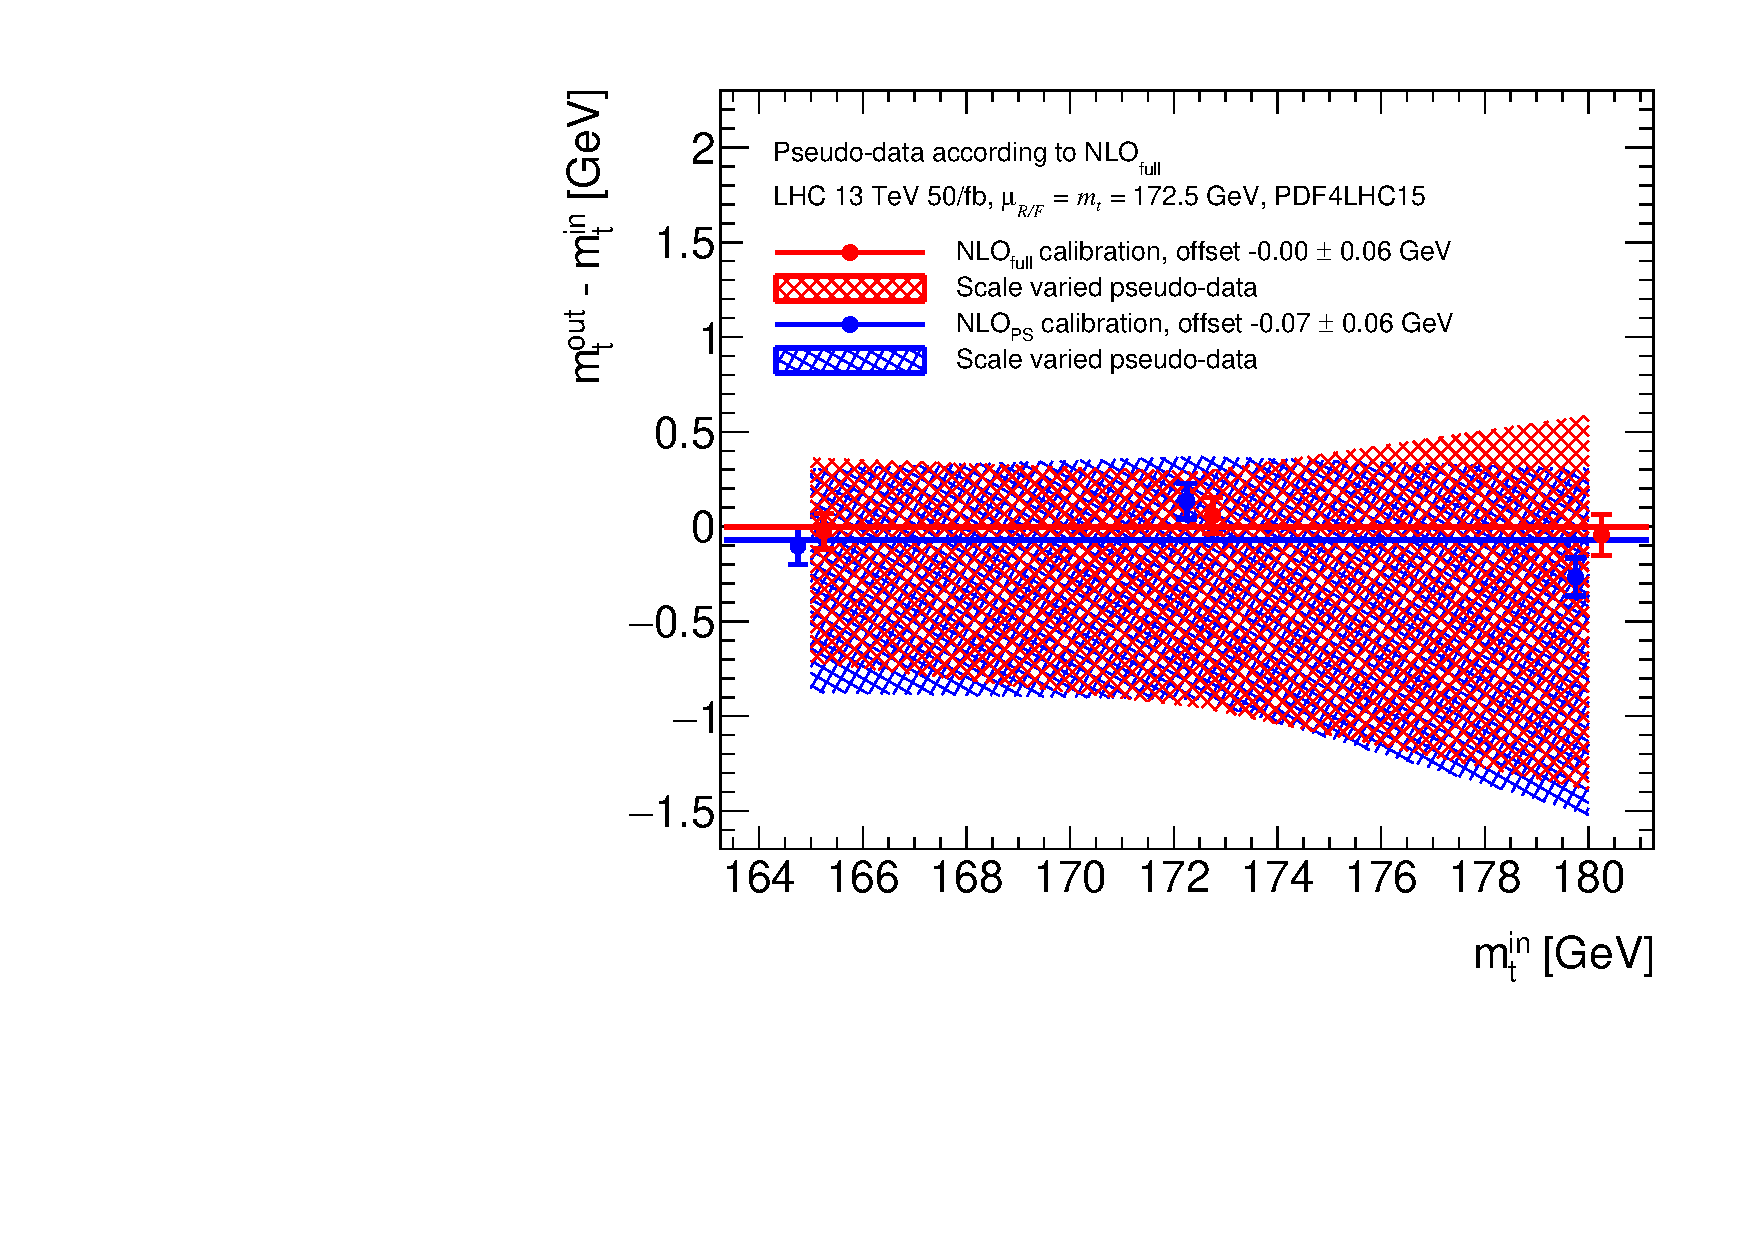
\includegraphics[width=\textwidth]{{plots/mt2_f1_13TeVstd_WWbb_NLO_vs_PS_pexpseed0}.pdf}
\vspace{\TwoFigBottom em}
\caption{\label{fig:WWbb_vs_PS_NLO_mt2}}
\end{subfigure}
\caption{\label{fig:NLO_WWbb_vs_mt2}%
  Same as Fig.~\ref{fig:NLO_WWbb_vs} but for the observable $m_{T2}$.}
\end{figure}


\begin{figure}[tbp!]
\centering
\begin{subfigure}{0.495\textwidth}
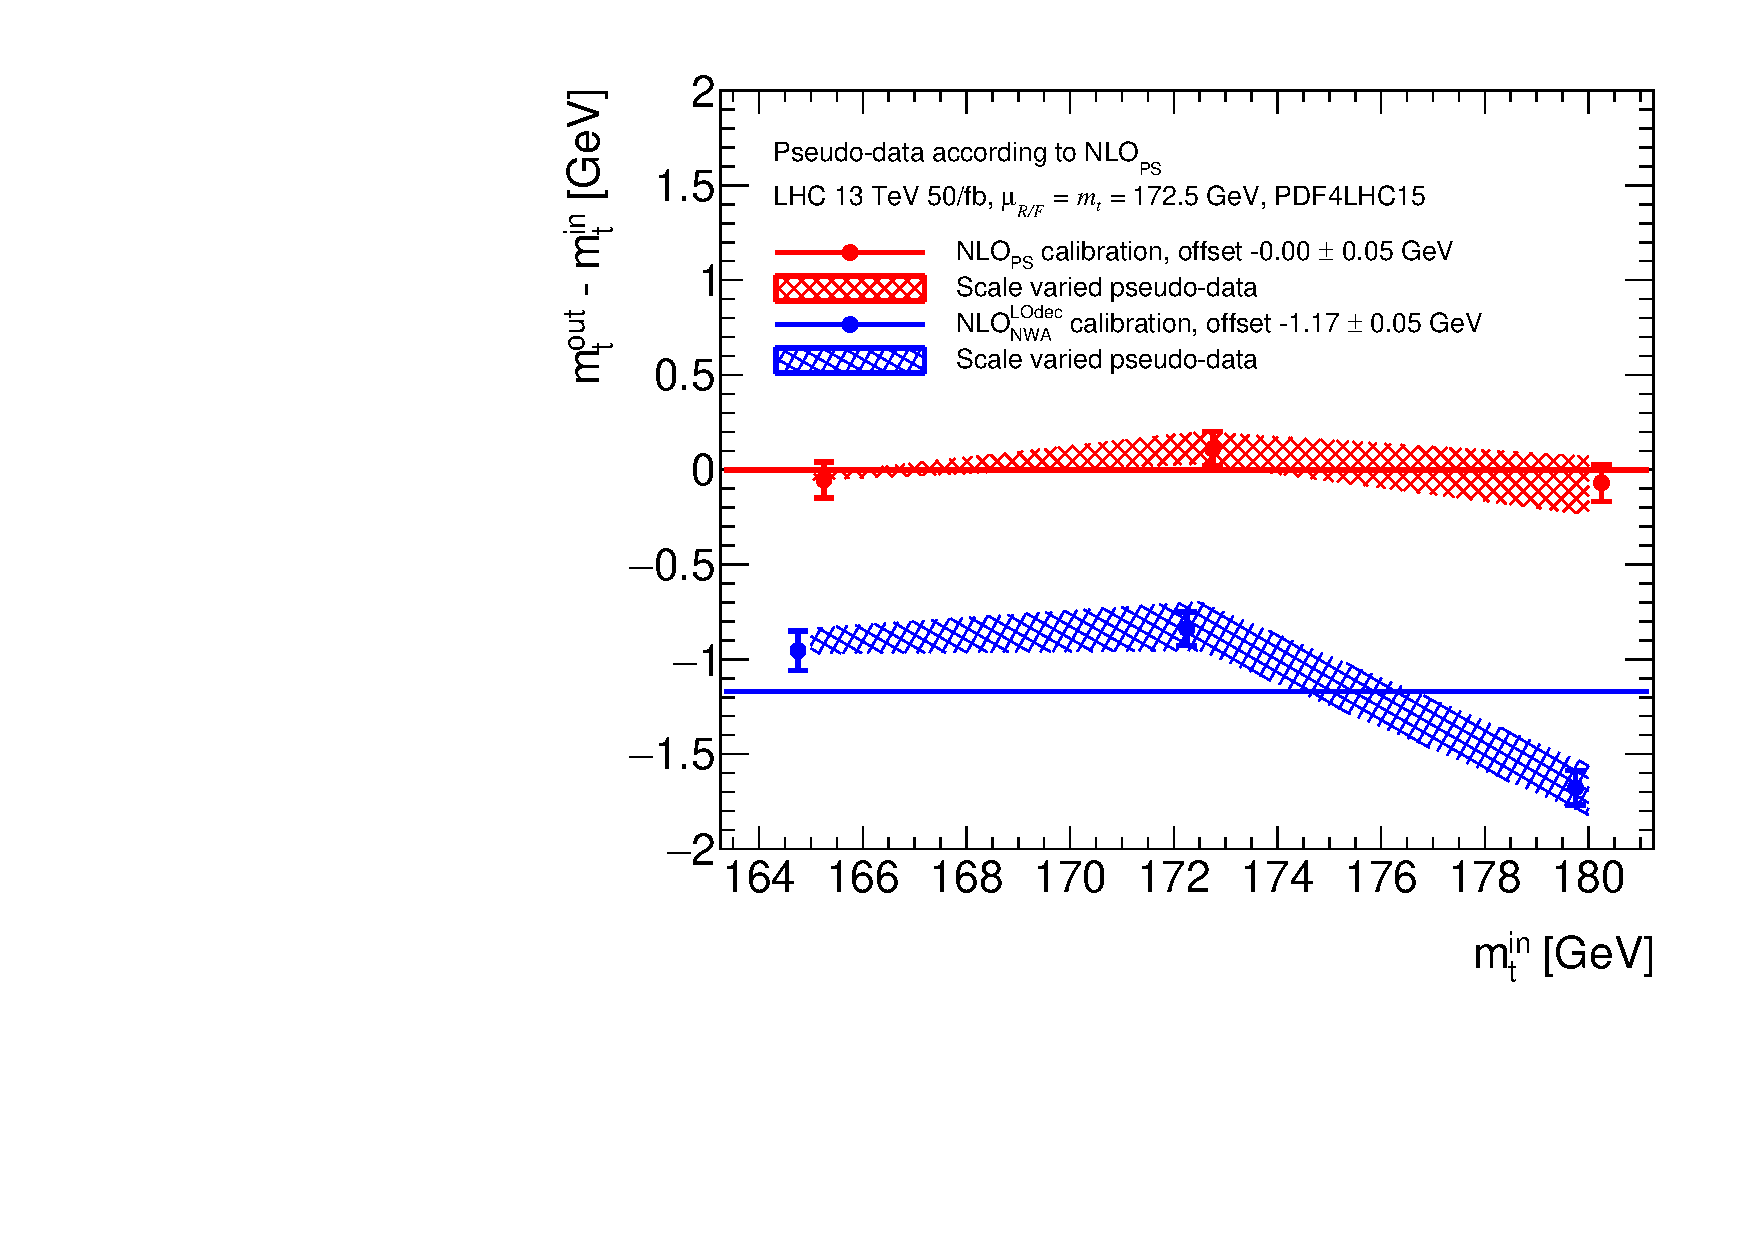
\includegraphics[width=\textwidth]{{plots/mt2_f1_13TeVstd_PS_vs_ttbar_NLO_pexpseed0}.pdf}
\vspace{\TwoFigBottom em}
\caption{\label{fig:PS_vs_ttbar_NLO_mt2}}
\end{subfigure}
\hfill
\begin{subfigure}{0.495\textwidth}
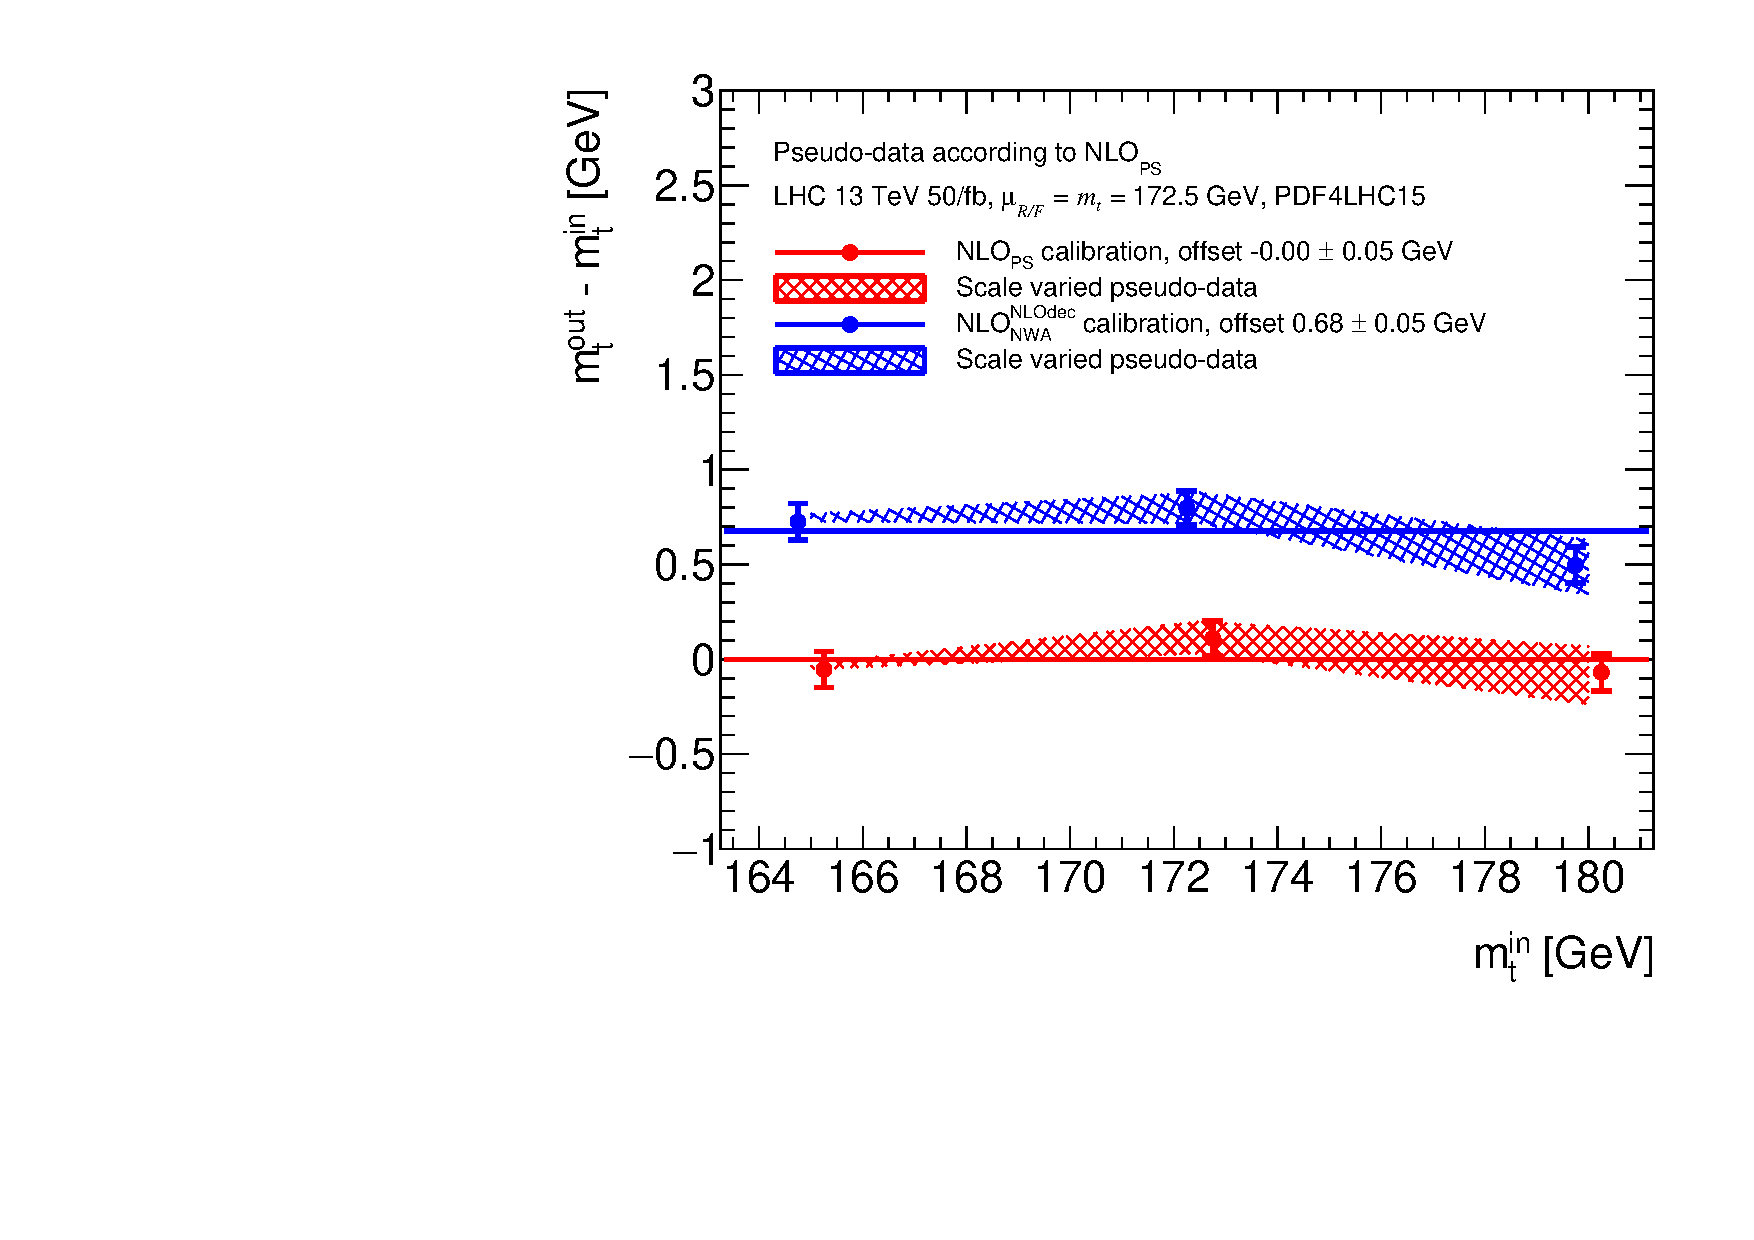
\includegraphics[width=\textwidth]{{plots/mt2_f1_13TeVstd_PS_vs_ttbar_NLO_nlodc_pexpseed0}.pdf}
\vspace{\TwoFigBottom em}
\caption{\label{fig:PS_vs_ttbar_NLO_nlodc_mt2}}
\end{subfigure}
\caption{\label{fig:NLO_PS_vs_mt2}%
  Same as Fig.~\ref{fig:NLO_PS_vs} but for the observable $m_{T2}$.}
\end{figure}

\begin{figure}[tbp!]
\centering
\begin{subfigure}{0.495\textwidth}
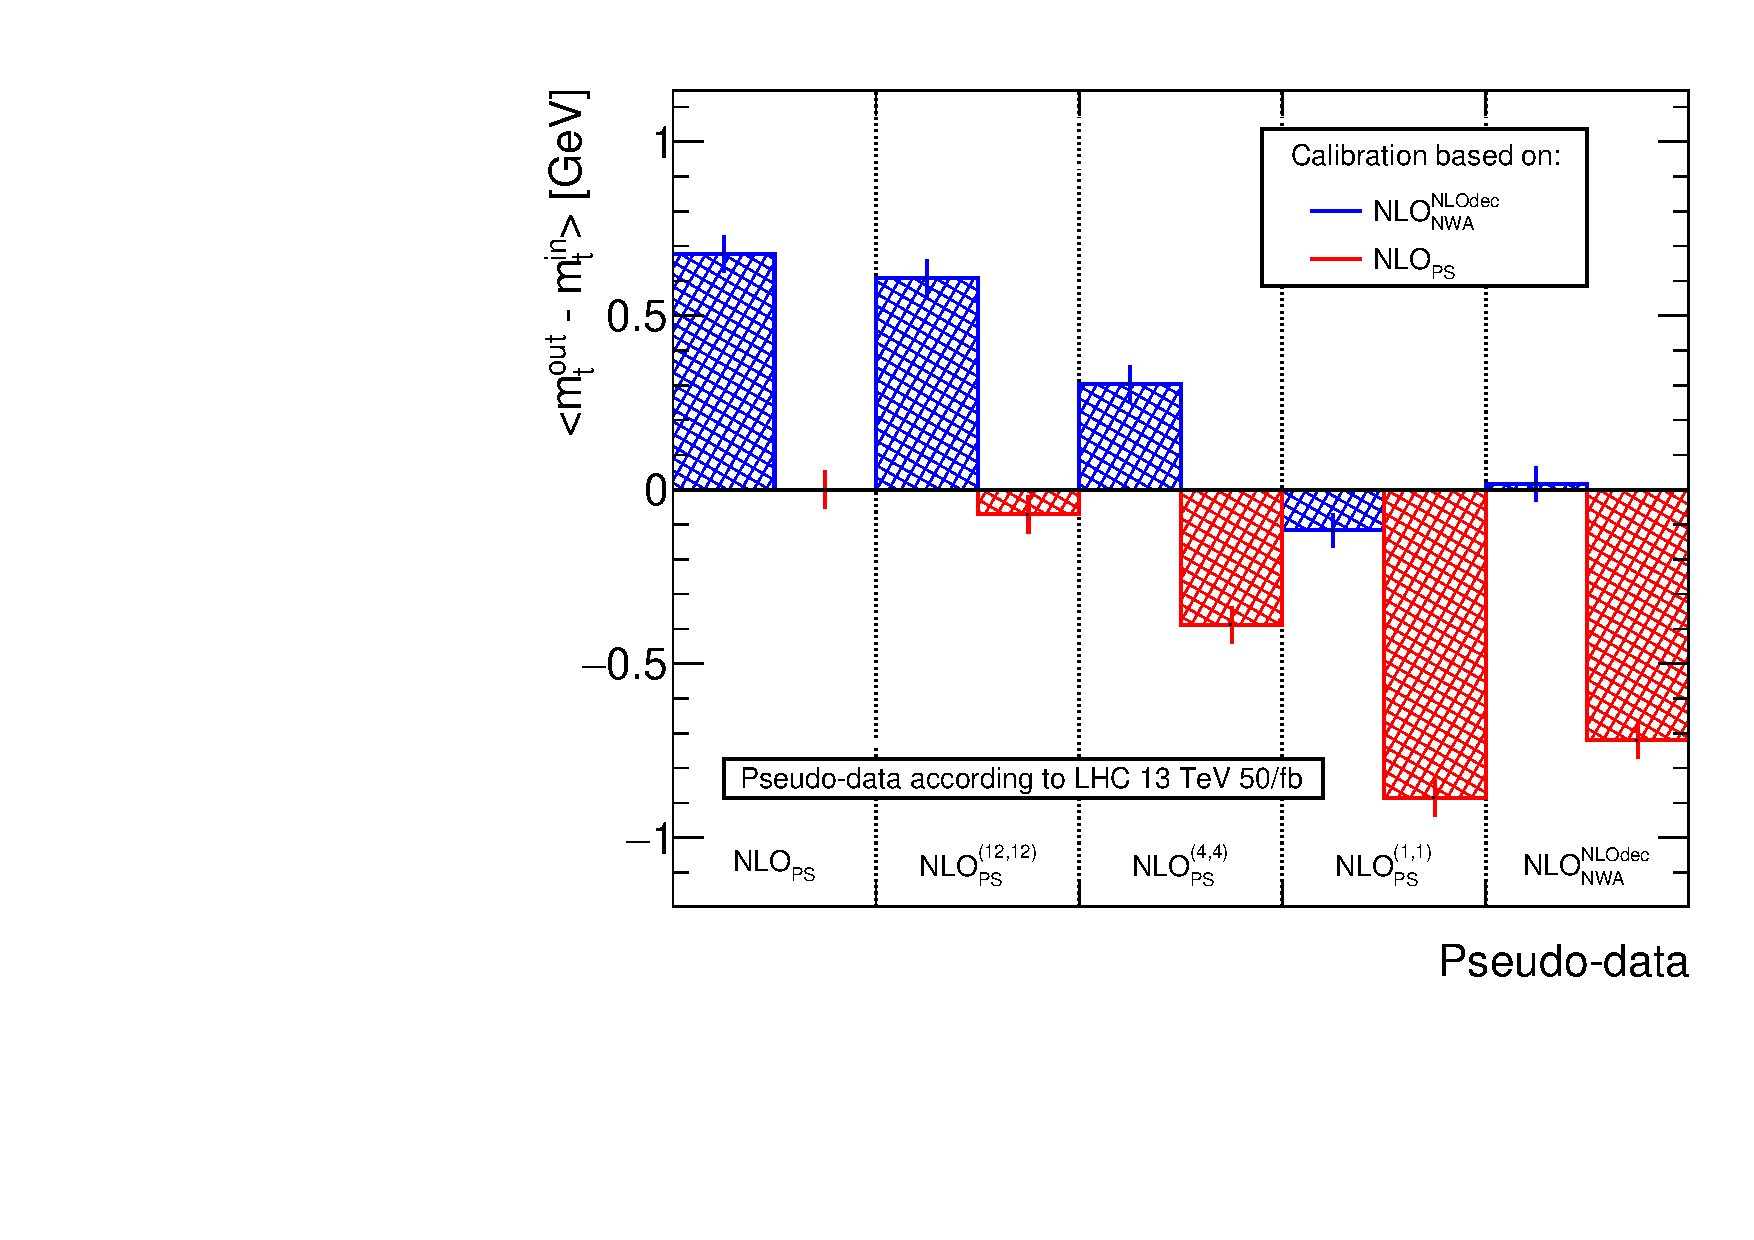
\includegraphics[width=\textwidth]{{plots/mt2_f1_DecOffsets_offset_pexpseed0}.pdf}
\vspace{\TwoFigBottom em}
\caption{\label{fig:oneemit_showers_var_mt2}}
\end{subfigure}
\hfill
\begin{subfigure}{0.495\textwidth}
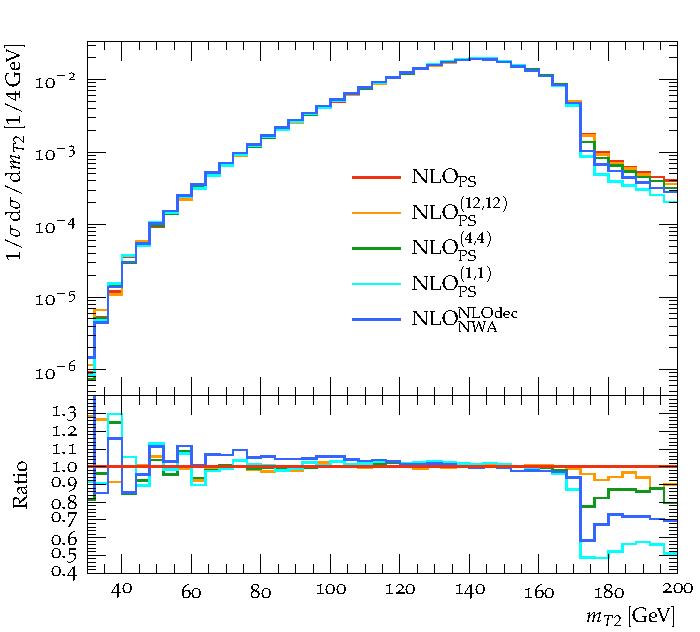
\includegraphics[width=\textwidth]{{plots/psrestricted.mt2}.pdf}
\vspace{\TwoFigBottom em}
\caption{\label{fig:oneemit_showers_var_mt2_dist}}
\end{subfigure}
\caption{\label{fig:oneemit_showers_mt2}%
  Same as Fig.~\ref{fig:oneemit_showers} but for the observable $m_{T2}$.}
\end{figure}

\begin{figure}[tbp!]
\centering
\begin{subfigure}{0.495\textwidth}
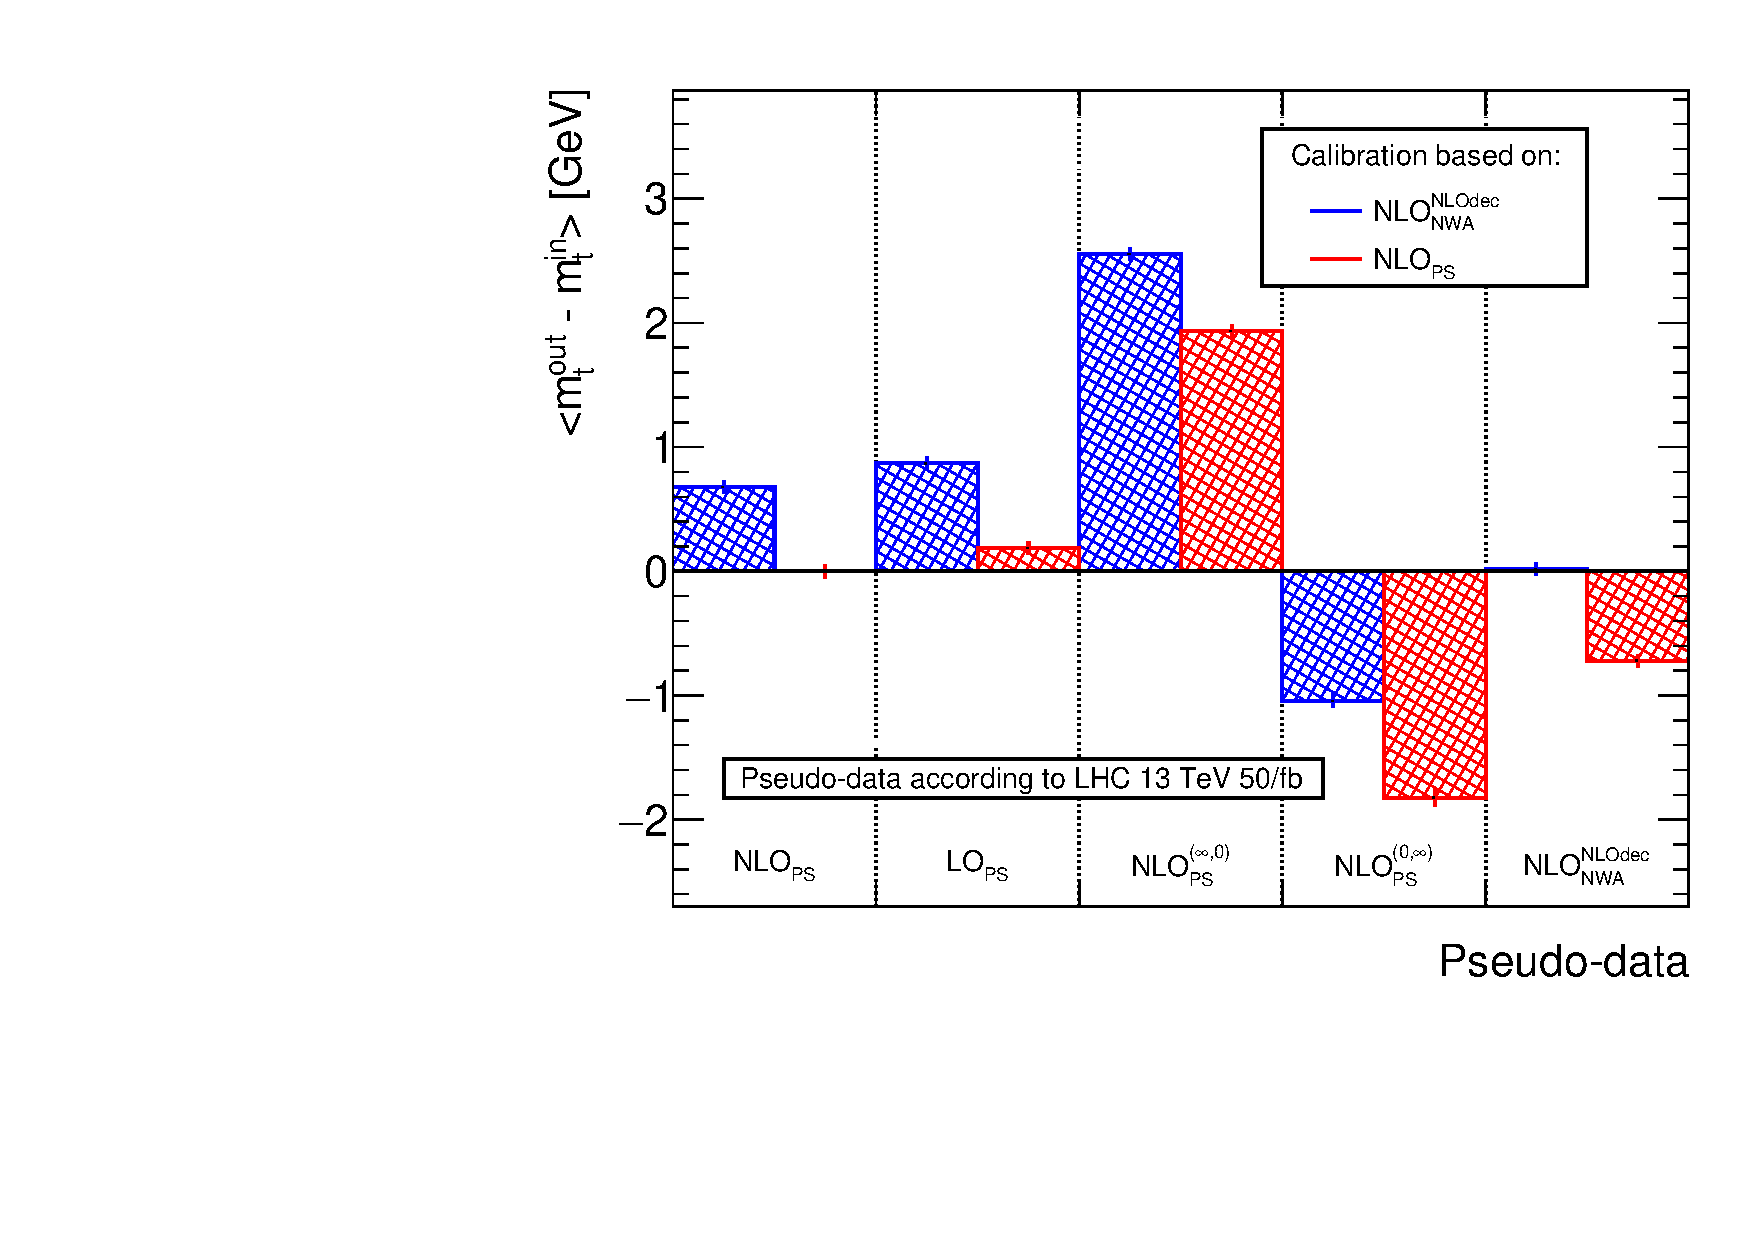
\includegraphics[width=\textwidth]{{plots/mt2_f1_DecOffsetsPure_offset_pexpseed0}.pdf}
\vspace{\TwoFigBottom em}
\caption{\label{fig:lo-prod-dec_showers_var_mt2}}
\end{subfigure}
\hfill
\begin{subfigure}{0.495\textwidth}
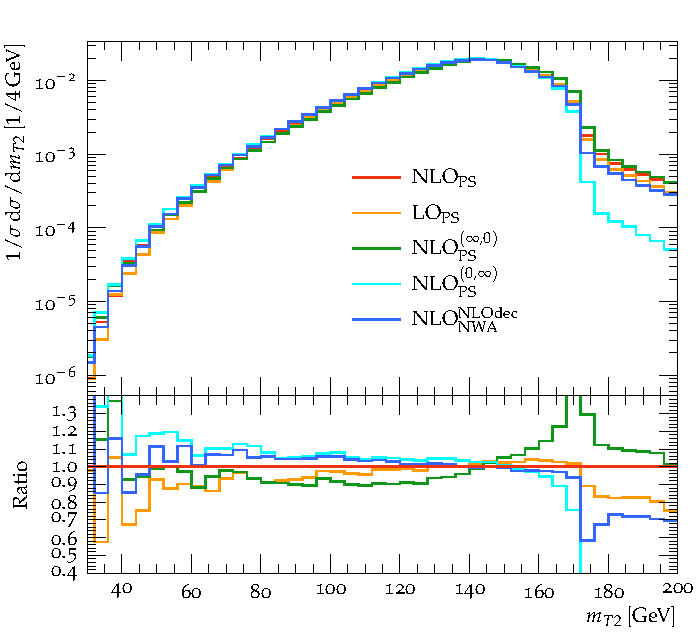
\includegraphics[width=\textwidth]{{plots/proddecay.mt2}.pdf}
\vspace{\TwoFigBottom em}
\caption{\label{fig:lo-prod-dec_showers_var_mt2_dist}}
\end{subfigure}
\caption{\label{fig:lo-prod-dec_showers_mt2}%
  Same as Fig.~\ref{fig:lo-prod-dec_showers} but for the observable $m_{T2}$.}
\end{figure}

\clearpage

\begin{figure}[tbp!]
\centering
\begin{subfigure}{0.495\textwidth}
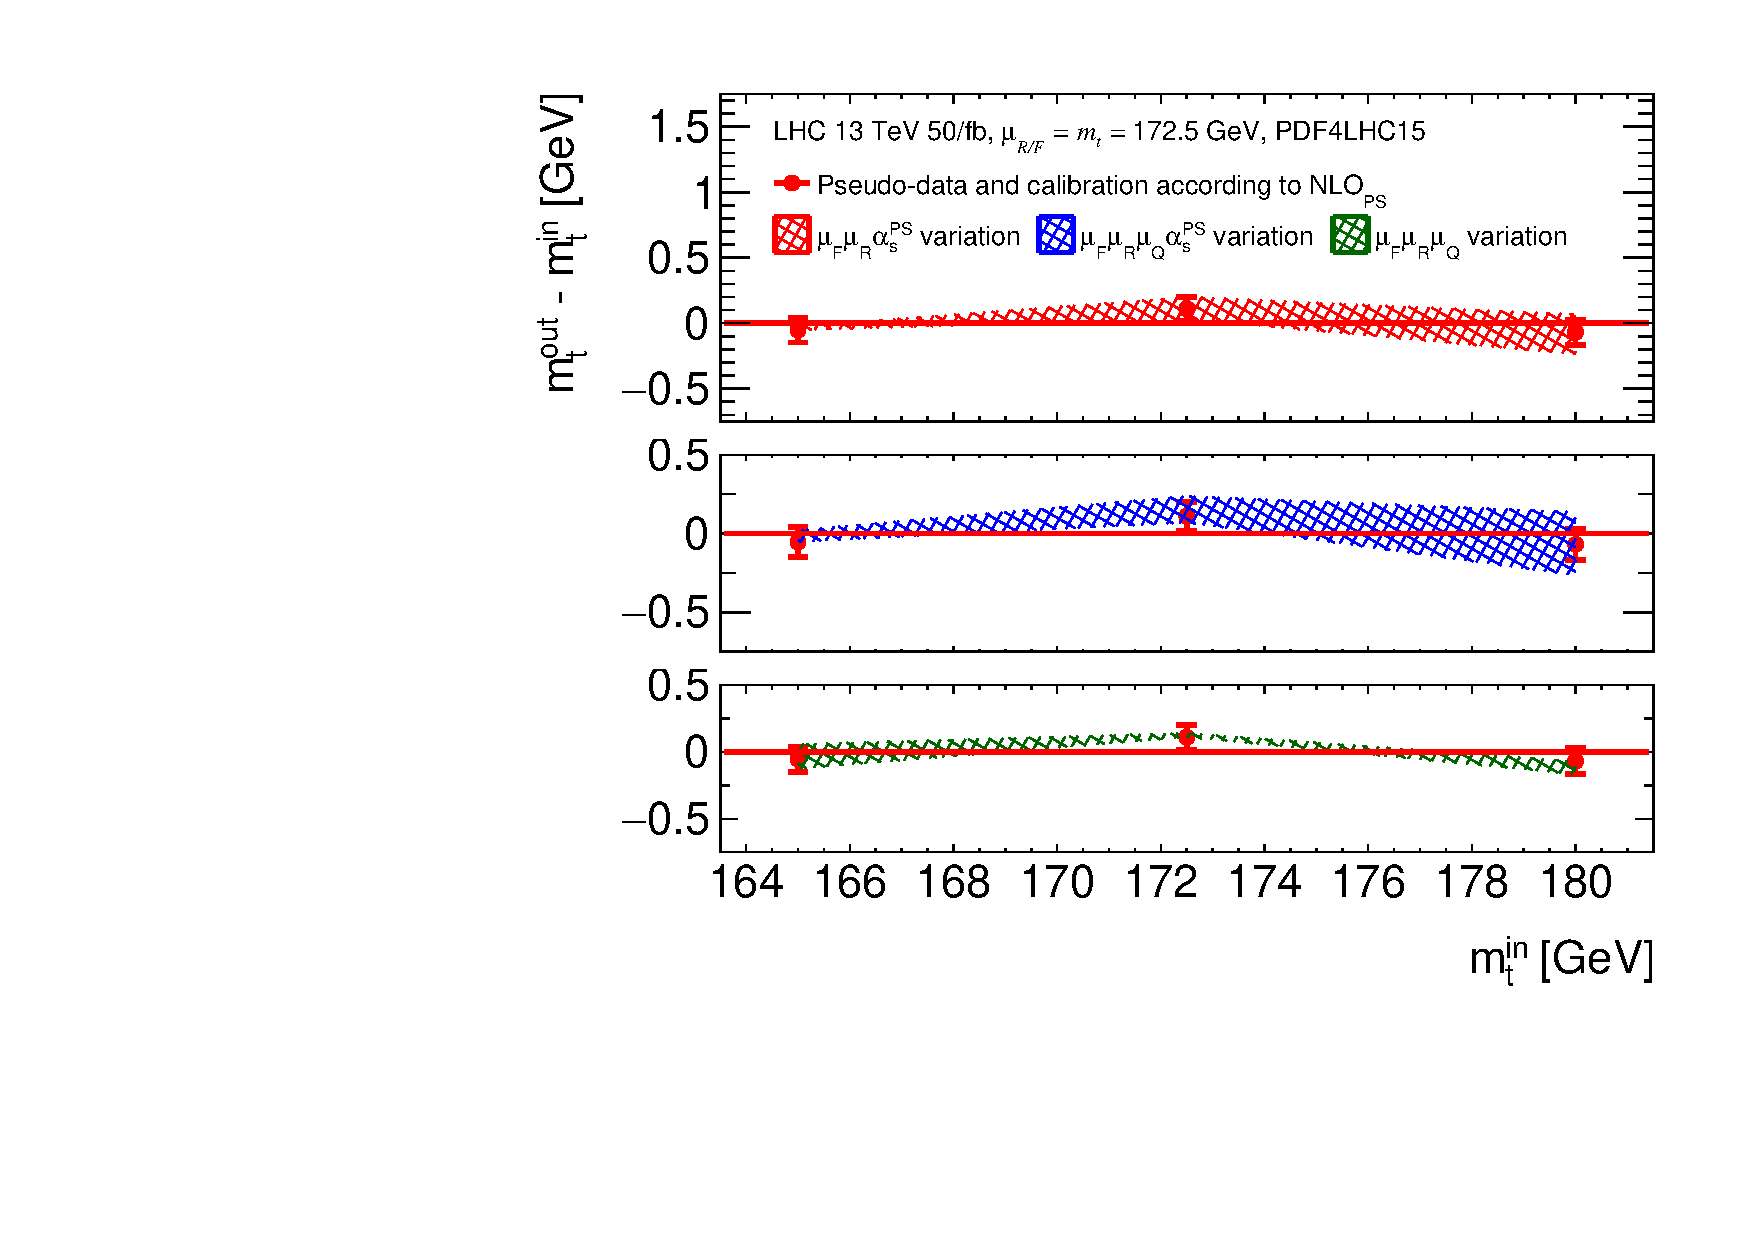
\includegraphics[width=\textwidth]{{plots/mt2_f1_PSvars_NLO_pexpseed0}.pdf}
\vspace{\TwoFigBottom em}
\caption{\label{fig:PS_scale_var_mt2}}
\end{subfigure}
\hfill
\begin{subfigure}{0.495\textwidth}
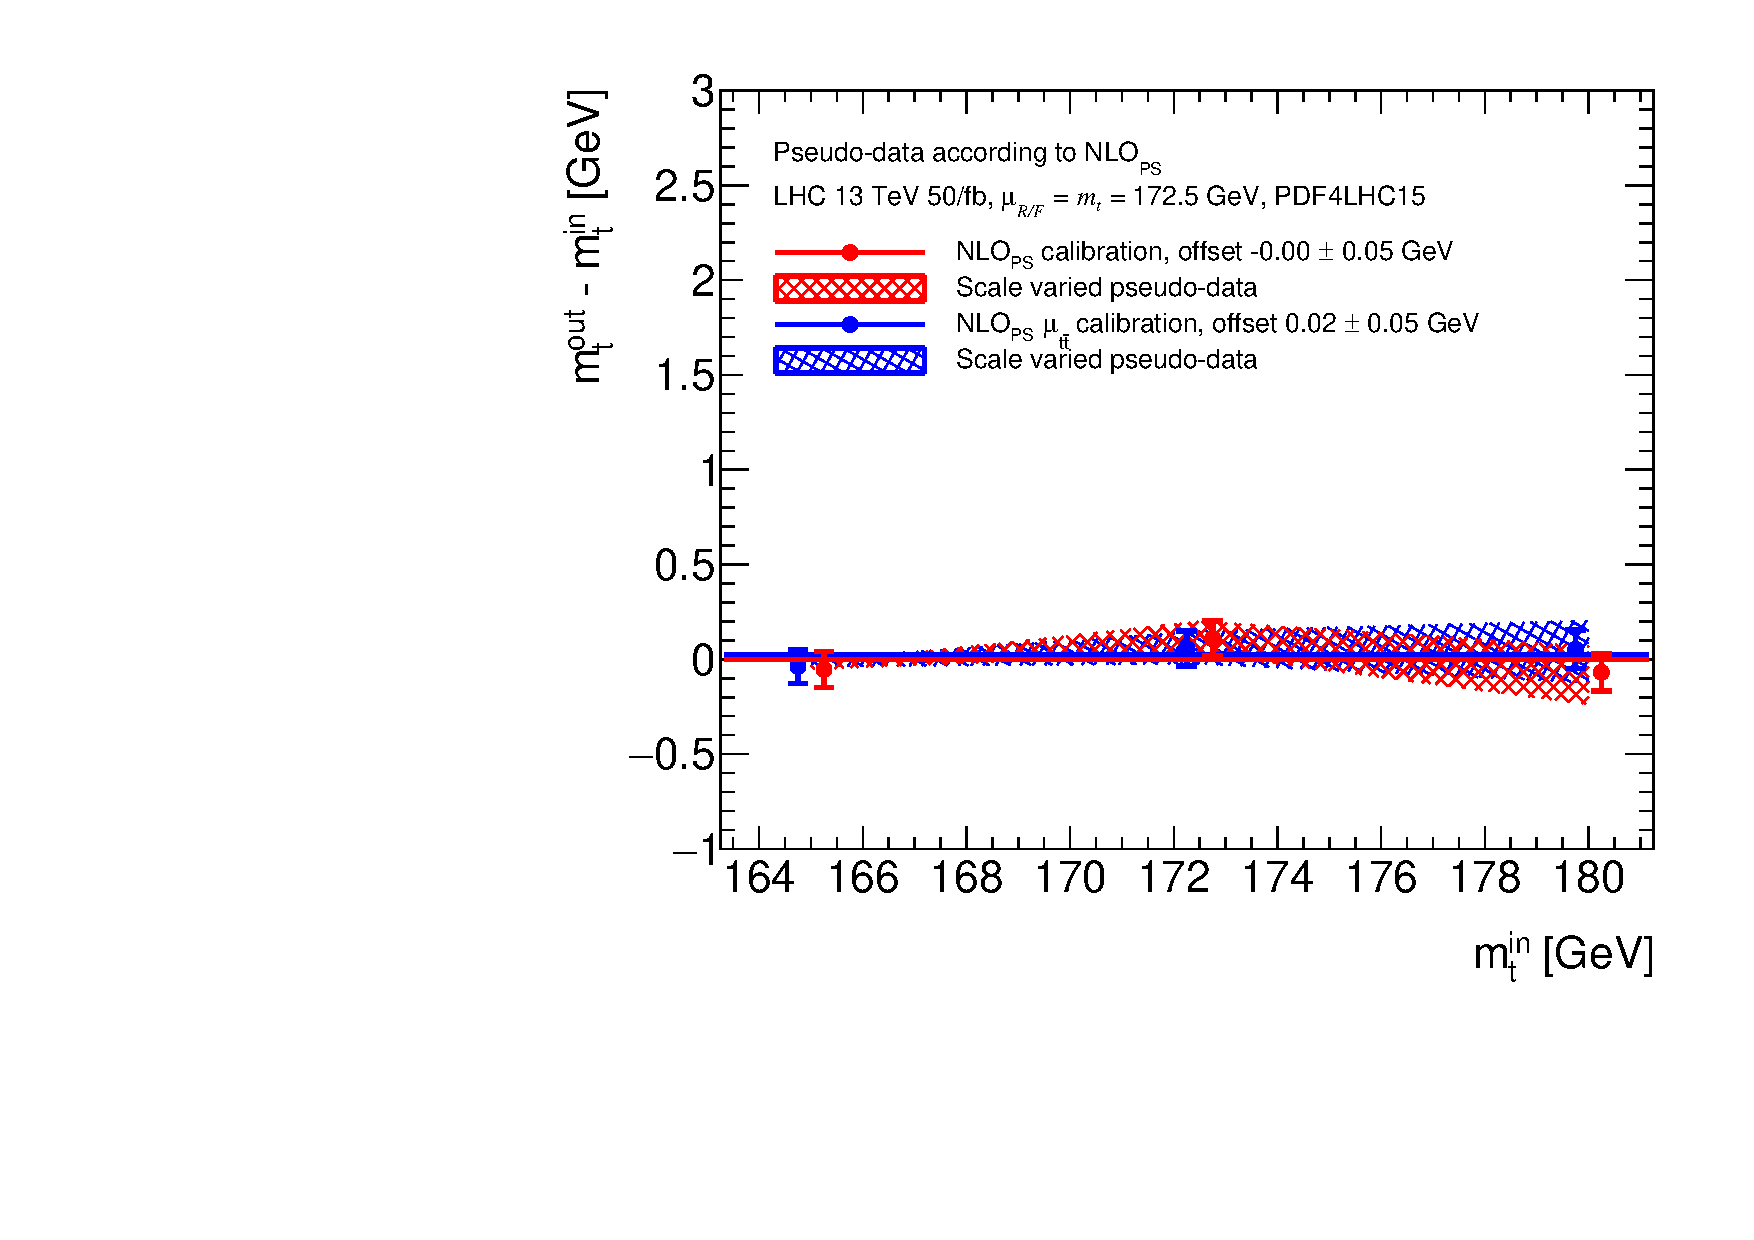
\includegraphics[width=\textwidth]{{plots/mt2_f1_13TeVstd_PS_scale_NLO_pexpseed0}.pdf}
\vspace{\TwoFigBottom em}
\caption{\label{fig:PS_scale_NLO_mt2}}
\end{subfigure}
\caption{\label{fig:PS_scale_mt2}%
  Same as Fig.~\ref{fig:PS_scale} but for the observable $m_{T2}$.
}
\end{figure}
